
\documentclass[a4paper,12pt,twoside]{report}
\usepackage[left=3cm,right=2cm,top=4cm,bottom=3cm]{geometry}
\usepackage[utf8]{inputenc}
\usepackage[spanish]{babel}
\usepackage{amsthm}
\usepackage{amsmath}
\usepackage{amsfonts}
\usepackage{pgf,tikz}
\usepackage{graphicx}
\usepackage{float}
\usepackage{cite}
\usepackage{enumerate}
\usepackage{courier}
\usepackage{listings}
\usepackage{color}
\usepackage{circuitikz}
\usetikzlibrary{arrows}
\definecolor{codegreen}{rgb}{0,0.6,0}
\definecolor{codegray}{rgb}{0.5,0.5,0.5}
\definecolor{codepurple}{rgb}{0.58,0,0.82}
\definecolor{backcolour}{rgb}{0.95,0.95,0.92}

\lstdefinestyle{mystyle}{
	backgroundcolor=\color{backcolour},   
	commentstyle=\color{codegreen},
	keywordstyle=\color{magenta},
	numberstyle=\tiny\color{codegray},
	stringstyle=\color{codepurple},
	basicstyle=\footnotesize\ttfamily,
	breakatwhitespace=false,         
	breaklines=true,                 
	captionpos=b,                    
	keepspaces=true,                 
	numbers=left,                    
	numbersep=5pt,                  
	showspaces=false,                
	showstringspaces=false,
	showtabs=false,                  
	tabsize=2
}

\lstset{style=mystyle}
\usepackage{hyperref}
\graphicspath{ {/home/booort/Escritorio/Fisymat/images/} }
\usepackage[toc,page]{appendix}


\documentclass[a4paper,12pt,twoside]{report}
\usepackage[left=3cm,right=2cm,top=4cm,bottom=3cm]{geometry}
\usepackage[utf8]{inputenc}
\usepackage[spanish]{babel}
\usepackage{amsthm}
\usepackage{amsmath}
\usepackage{amsfonts}
\usepackage{pgf,tikz}
\usepackage{graphicx}
\usepackage{float}
\usepackage{cite}
\usepackage{enumerate}
\usepackage{courier}
\usepackage{listings}
\usepackage{color}
\usepackage{circuitikz}
\usetikzlibrary{arrows}
\definecolor{codegreen}{rgb}{0,0.6,0}
\definecolor{codegray}{rgb}{0.5,0.5,0.5}
\definecolor{codepurple}{rgb}{0.58,0,0.82}
\definecolor{backcolour}{rgb}{0.95,0.95,0.92}

\lstdefinestyle{mystyle}{
	backgroundcolor=\color{backcolour},   
	commentstyle=\color{codegreen},
	keywordstyle=\color{magenta},
	numberstyle=\tiny\color{codegray},
	stringstyle=\color{codepurple},
	basicstyle=\footnotesize\ttfamily,
	breakatwhitespace=false,         
	breaklines=true,                 
	captionpos=b,                    
	keepspaces=true,                 
	numbers=left,                    
	numbersep=5pt,                  
	showspaces=false,                
	showstringspaces=false,
	showtabs=false,                  
	tabsize=2
}

\lstset{style=mystyle}
\usepackage{hyperref}
\graphicspath{ {/home/booort/Escritorio/Fisymat/images/} }
\usepackage[toc,page]{appendix}


\documentclass[a4paper,12pt,twoside]{report}
\usepackage[left=3cm,right=2cm,top=4cm,bottom=3cm]{geometry}
\usepackage[utf8]{inputenc}
\usepackage[spanish]{babel}
\usepackage{amsthm}
\usepackage{amsmath}
\usepackage{amsfonts}
\usepackage{pgf,tikz}
\usepackage{graphicx}
\usepackage{float}
\usepackage{cite}
\usepackage{enumerate}
\usepackage{courier}
\usepackage{listings}
\usepackage{color}
\usepackage{circuitikz}
\usetikzlibrary{arrows}
\definecolor{codegreen}{rgb}{0,0.6,0}
\definecolor{codegray}{rgb}{0.5,0.5,0.5}
\definecolor{codepurple}{rgb}{0.58,0,0.82}
\definecolor{backcolour}{rgb}{0.95,0.95,0.92}

\lstdefinestyle{mystyle}{
	backgroundcolor=\color{backcolour},   
	commentstyle=\color{codegreen},
	keywordstyle=\color{magenta},
	numberstyle=\tiny\color{codegray},
	stringstyle=\color{codepurple},
	basicstyle=\footnotesize\ttfamily,
	breakatwhitespace=false,         
	breaklines=true,                 
	captionpos=b,                    
	keepspaces=true,                 
	numbers=left,                    
	numbersep=5pt,                  
	showspaces=false,                
	showstringspaces=false,
	showtabs=false,                  
	tabsize=2
}

\lstset{style=mystyle}
\usepackage{hyperref}
\graphicspath{ {/home/booort/Escritorio/Fisymat/images/} }
\usepackage[toc,page]{appendix}


\documentclass[a4paper,12pt,twoside]{report}
\usepackage[left=3cm,right=2cm,top=4cm,bottom=3cm]{geometry}
\usepackage[utf8]{inputenc}
\usepackage[spanish]{babel}
\usepackage{amsthm}
\usepackage{amsmath}
\usepackage{amsfonts}
\usepackage{pgf,tikz}
\usepackage{graphicx}
\usepackage{float}
\usepackage{cite}
\usepackage{enumerate}
\usepackage{courier}
\usepackage{listings}
\usepackage{color}
\usepackage{circuitikz}
\usetikzlibrary{arrows}
\definecolor{codegreen}{rgb}{0,0.6,0}
\definecolor{codegray}{rgb}{0.5,0.5,0.5}
\definecolor{codepurple}{rgb}{0.58,0,0.82}
\definecolor{backcolour}{rgb}{0.95,0.95,0.92}

\lstdefinestyle{mystyle}{
	backgroundcolor=\color{backcolour},   
	commentstyle=\color{codegreen},
	keywordstyle=\color{magenta},
	numberstyle=\tiny\color{codegray},
	stringstyle=\color{codepurple},
	basicstyle=\footnotesize\ttfamily,
	breakatwhitespace=false,         
	breaklines=true,                 
	captionpos=b,                    
	keepspaces=true,                 
	numbers=left,                    
	numbersep=5pt,                  
	showspaces=false,                
	showstringspaces=false,
	showtabs=false,                  
	tabsize=2
}

\lstset{style=mystyle}
\usepackage{hyperref}
\graphicspath{ {/home/booort/Escritorio/Fisymat/images/} }
\usepackage[toc,page]{appendix}

\include{thesis.preamble}


\begin{document}
	


\title{\LARGE {\bf Ejercicios de Redes complejas en fisica y neurociencia}\\
 \vspace*{6mm}
}

\author{Bartolomé Ortiz Viso}
\submitdate{Mayo 2018}

\narrowlinespacing
\maketitle

\preface
\input{abstract/abstract}


\body
\input{tema1/tema1.tex}
\input{tema2/tema2.tex}
\input{tema4/tema4.tex}
\input{tema6/tema6.tex}



\appendix
\input{tema1/tema1code.tex}
\input{tema2/tema2code.tex}
\input{tema4/tema3code.tex}
\input{tema6/tema4code.tex}



\end{document}



\begin{document}
	


\title{\LARGE {\bf Ejercicios de Redes complejas en fisica y neurociencia}\\
 \vspace*{6mm}
}

\author{Bartolomé Ortiz Viso}
\submitdate{Mayo 2018}

\narrowlinespacing
\maketitle

\preface

\addcontentsline{toc}{chapter}{Abstract}

\begin{abstract}

Este trabajo compone la resolucion de algunos de los ejercicios propuestos en la asignatura del Master de Fisica y Matematicas fisymat de la Universidad de Granada denominada Fisica de redes complejas. La primera parte de la asignatura es impartida por el profesor Joaquín Torres. 

Generalmente la mayoría de los ejercicios poseen algún componente computacional, ya sean cálculos, simulación o visualización. Con el fin de resaltar la importancia de este aspecto, pero no dificultar la lectura, los códigos están adjuntos y se pueden consultar en los apéndices dejando solo para el grueso del texto las conclusiones derivadas y las visualizaciones. 

Así mismo muchos de los códigos empleados tambien poseen un salida visual en forma de animaciones y videos que puede ser interesante observar. Para este fin puede consultar el respositorio en github donde están todos los códigos utilizados, las salidas de los mismos y por supuesto, una versión de este documento en pdf y latex bajo la licencia creative commons:

\url{http://www.github.com/thebooort/Complex-Networks-and-Neuroscience}
 
 Algunos de los códigos utilizados utilizan partes de otras librerías o códigos. En esos casos quedan citados los otros responsables y la licencia se adhiere a la que pusieran sus creadores iniciales antes de mis modificaciones para este trabajo.
 

\end{abstract}



\body
\chapter{Sistemas complejos}
\section{Atractores}
\subsubsection{\large Simular y analizar el comportamiento complejo del atrayente de Lorenz} 
El descubrimiento de este atractor data de 1963, cuando Edward Norton Lorenz desarrolló un modelo matemático simplificado para la convección atmosférica. El modelo es un sistema de ecuaciones diferenciales ordinarias compuesto por tres ecuaciones ahora conocidas como las ecuaciones de Lorenz:
$$\left\{\begin{matrix}\frac{\mathrm{d}x}{\mathrm{d}t} &= \sigma (y - x), \\
	\frac{\mathrm{d}y}{\mathrm{d}t} &= x (\rho - z) - y, \\
	\frac{\mathrm{d}z}{\mathrm{d}t} &= x y - \beta z.\end{matrix}\right.$$
Normalmente se asume que los parametros $\sigma$, $\rho$, y $\beta$ son positivos. El interés en este modelo proviene de que para una seleccion de valores como $\sigma = 10$, $\beta = 8/3$ and $\rho = 28 $ el sistema exhibe un comportamiento caótico.

Si $\rho < 1$ entonces sólo hay un punto de equilibrio en el origen. Este punto además es un atractor global.

Si $\rho = 1$ entonces la en nuestra dinámica aparece una bifurcacion de pitchfork , y para  $\rho > 1 $ apareceen dos puntos de equilibrio, a saber $\left( \sqrt{\beta(\rho-1)}, \sqrt{\beta(\rho-1)}, \rho-1 \right) $ and $\left( -\sqrt{\beta(\rho-1)}, -\sqrt{\beta(\rho-1)}, \rho-1 \right). $ 
Este par de puntos será estable si : $\rho < \sigma\frac{\sigma+\beta+3}{\sigma-\beta-1}$

Como avanzábamos para valores como $\rho = 28$, $\sigma = 10$, and $\beta = 8/3$, el sistema de Lorenz tiene soluciones caóticas (es decir que, aunque no todas las soluciones son caóticas algunas de ellas si pueden presentar este comportamiento).

 Casi todos los puntos iniciales tenderán a un conjunto invariable que es lo que denominamos el atractor de Lorenz (véase figura:\ref{lorentz1}), cuya forma geométrica es reconocible. Este comportamiento caótico se refleja en la gran sensibilidad del atractor frente a cambios en las condiciones iniciales como se puede ver en la grafica \ref{lorentz2}.\textit{ Las graficas pertenecen a extractos de animaciones que pueden consultarse en github.}
 
 \begin{figure}
 	\centering
 	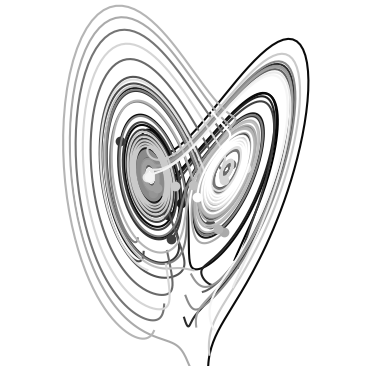
\includegraphics[width=8cm]{lorentz}
 	\caption{Atractor de Lorentz}
 	\label{lorentz1}
 \end{figure}
 \begin{figure}
 	\centering
 	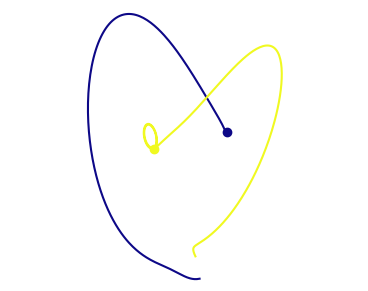
\includegraphics[width=8cm]{lorentz1}
 	\caption{Atractor de Lorentz: variacion respecto a condiciones iniciales}
 	\label{lorentz2}
 \end{figure}
 
 \subsubsection{\large Simular y analizar el comportamiento complejo del atrayente de Rossler} 
 
 El atractor de Rössler es el atractor del sistema de Rössler, un sistema de tres ecuaciones diferenciales ordinarias no lineales estudiadas por Otto E. Rössler. Estas ecuaciones diferenciales definen un sistema dinámico del tiempo-continuo que muestra dinámicas caóticas asociadas con las propiedades fractales del atractor:
 $$\left\{\begin{matrix}\frac{dx}{dt} &= -y - z \\
 \frac{dy}{dt} &= x + ay, \\
 \frac{dz}{dt} &= b + z(x-c).\end{matrix}\right.$$
 Rössler estudió el atractor caótico con $ a = 0.2 $, $ b = 0.2 $ y $ c = 5.7 $, aunque las propiedades de $ a = 0.1 $, $ b = 0.1 $, y $ c = 14 $ han sido más comúnmente utilizadas desde entonces.
 De nuevo con estos parámetros podemos encontrar orbitas con comportamiento caótico como se representa en la figura \ref{rossler1}. \textit{ La grafica pertenecen a extractos de animaciones que pueden consultarse en github.}
  \begin{figure}
  	\centering
  	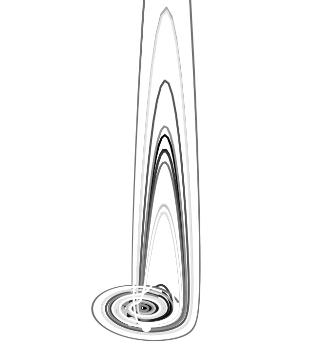
\includegraphics[width=8cm]{rossler}
  	\caption{Atractor de Rossler}
  	\label{rossler1}
  \end{figure}
  
 \section{Juego de la vida}
 \subsubsection{\large Simular el juego de la vida y estudiar su comportamiento emergente} 
  
  El juego de la vida es un autómata celular diseñado por el matemático británico John Horton Conway en 1970.
  
  Hizo su primera aparición pública en el número de octubre de 1970 de la revista Scientific American, en la columna de juegos matemáticos de Martin Gardner. Desde un punto de vista teórico, es interesante porque es equivalente a una máquina universal de Turing, es decir, todo lo que se puede computar algorítmicamente se puede computar en el juego de la vida.
    \begin{figure}
    	\centering
    	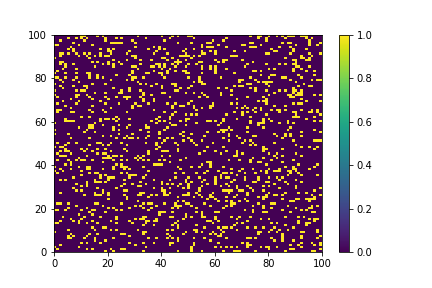
\includegraphics[width=8cm]{generation0}
    	\caption{Disposicion inicial: partimos de una distribucion aleatoria de puntos en una malla}
    	\label{gol1}
    \end{figure}
  \begin{figure}
  	\centering
  	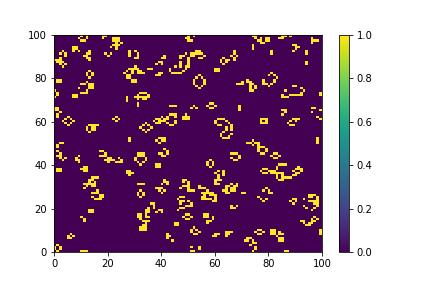
\includegraphics[width=8cm]{generation5}
  	\caption{Evolucion del juego de la vida tras 5 pasos temporale}
  	\label{gol2}
  \end{figure}
  \begin{figure}
  	\centering
  	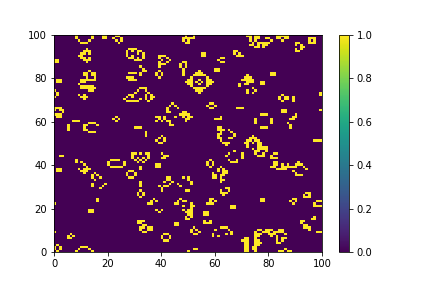
\includegraphics[width=8cm]{generation10}
  	\caption{Evolucion del juego de la vida tras 10 pasos temporales }
  	\label{gol3}
  \end{figure}
  Para profundizar un poco más en el trabajo se ha desarrollado un programa para detectar si patrones implementados generan naves espaciales.
  Las naves espaciales son patrones que reaparecen en otra posición tras completar su período. Esto es, son patrones que tras un número finito de generaciones vuelven a su estado original pero en una ubicación diferente.
  En este caso se han utilizado las reglas estándar. Tras 4 pasos temporales se localizó que la figura era una nave espacial (figuras \ref{gol4} y \ref{gol5})
   \begin{figure}
   	\centering
   	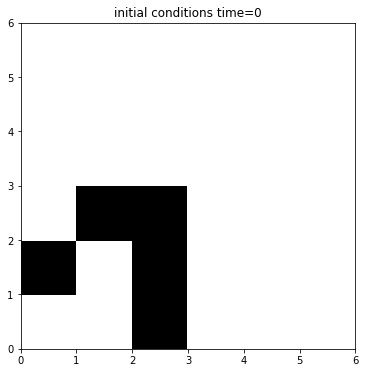
\includegraphics[width=8cm]{searcher_1}
   	\caption{Disposicion inicial encontrada como buena }
   	\label{gol4}
   \end{figure}
    \begin{figure}
    	\centering
    	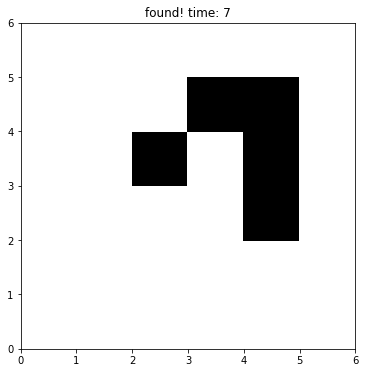
\includegraphics[width=8cm]{searcher_2}
    	\caption{Identidad identica transportadad tras 4 pasos temporales }
    	\label{gol5}
    \end{figure}
    Esta es la nave espacial más famosa, conocida como glider.
\subsubsection{\large Modelo pilas de arena}     
El modelo de pilas de arena es un modelo matemático diseñado para analizar y explicar el comportamiento de autoorganización crítica a través de la teoría de grafos y la teoría de autómatas celulares utilizando herramientas algebraicas.

Si consideramos un plano con una gran cantidad de arena al que se le va añadiendo un poco cada paso temporal, si la pendiente es muy alta, la arena tenderá a caer provocando una avalancha, pues es un estado insetable. Esto se poducirá hasta que todo llegue a un estado estable en cuanto a la pendiente.

Se pueden ver el resultado de las simulaciones en \ref{sand1},\ref{sand2},\ref{sand3}

 \begin{figure}
 	\centering
 	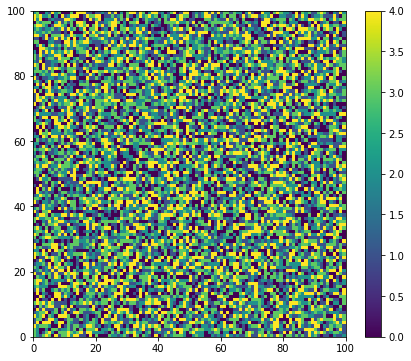
\includegraphics[width=8cm]{pila_arena_random}
 	\caption{Pila de arena con condiciones iniciales aleatorias  }
 	\label{sand1}
 \end{figure}
  \begin{figure}
  	\centering
  	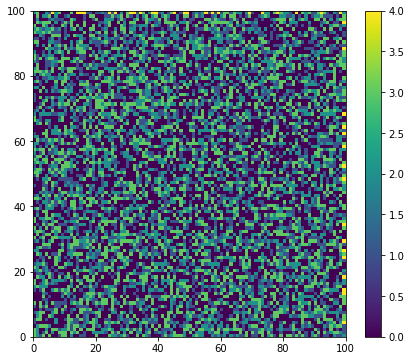
\includegraphics[width=8cm]{pila_arena_random_2}
  	\caption{Sin adicion y partiendo de \ref{sand1} vemos como el sistema tiene a producir avalanchas hasta nivelarse }
  	\label{sand2}
  \end{figure}

 \begin{figure}
 	\centering
 	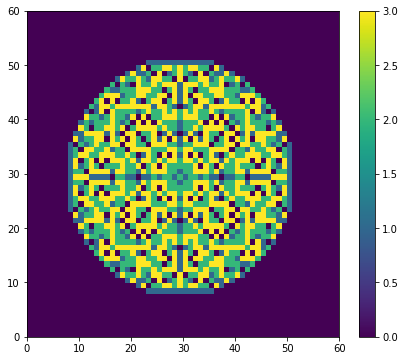
\includegraphics[width=8cm]{pila_arena}
 	\caption{Creacion de fractales cuando añadimos un goteo de arena en el centro durante 100 pasos de tiempo }
 	\label{sand3}
 \end{figure}


    
\subsubsection{\large Modelo hormiga de langton}    
Aunque no partía como ejercicio, buscando información sobre algunas de turing y el juego de la vida también he encontrado otra sencilla maquina con comportamientos emergentes que dejo a continuación.
La hormiga de Langton es un una máquina de Turing bidimensional con un conjunto de reglas muy sencillo, que sin embargo da lugar a comportamientos emergentes complejos.
 La hormiga de Langton clásica opera sobre una rejilla espacial cuadrada, en que cada celda puede estar en uno de dos estados (blanca o negra, 1 o 0, viva o muerta, etc). Fue inventada por Chris Langton en 1986 y su universalidad se demostró en el año 2000.
 
 La hormiga siempre está mirando en una de las cuatro direcciones cardinales y se mueve un cuadrado cada vez, de acuerdo con las siguientes reglas:
 \begin{itemize}
 	\item Si está sobre un cuadrado blanco, cambia el color del cuadrado, gira noventa grados a la izquierda y avanza un cuadrado.
 	\item Si está sobre un cuadrado negro, cambia el color del cuadrado, gira noventa grados a la derecha y avanza un cuadrado.
 \end{itemize}
 
   \begin{figure}
   	\centering
   	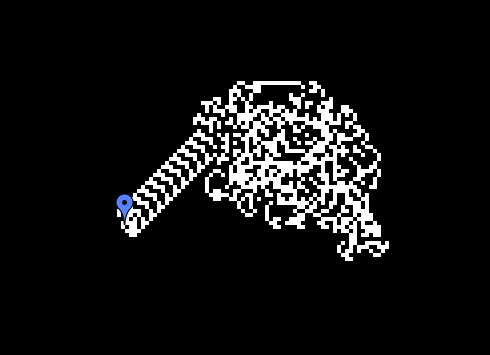
\includegraphics[width=8cm]{ant}
   	\caption{Hormiga tras 11000 pasos temporales. Las condiciones iniciales son nulas salvo la casilla de la hormiga }
   	\label{ant}
   \end{figure}
  



\section{Dimensiones de Haussdorf: variedades continuas y fractales}
\subsubsection{\large Demostrar que con la definición de dimension de Haussdorf se tiene (para variedades continuas:curva, superficie, y volumen) las dimensiones esperadas.} 

Partimos de la formula descrita en los apuntes, la dimension de Haussdorf ($D$) de una variedad viene determinada por:
\begin{equation}
D=\lim_{a\rightarrow 0}(\frac{-ln(N(a))}{ln(a)})
\end{equation}
donde $N(a)$ es el número mínimo de $esferas$ $d–dimensionales$ necesarias para cubrir por completo la variedad en cuestión.
Teniendo en cuenta que $d T \leq D \leq d$, donde $d$ es la dinemsion euclídea y $d_T$ e sla dimension topológica, sabemos de antemano que como todas nuestras variedades son continuas, el valor será $1,2,3$ para la curva, la superficie y le columen, respectivamente. Analizamos caso por caso: 
\begin{itemize}
	\item Curva continua:
	
	En este caso las $esferas$ $d–dimensionales$ son segmentos de longitud $2a$, por tanto, sea una curva continua con longitud $1$:
	\begin{equation}
	\begin{split}
	D=\lim_{a\rightarrow 0}(\frac{-ln(N(a))}{ln(a)})
	&=-\lim_{a\rightarrow 0}(\frac{ln(1/2a)}{ln(a)})\\
	=-\lim_{a\rightarrow 0}(\frac{\frac{d}{da}ln(1/2a)}{\frac{d}{da}ln(a)})
	&=-\lim_{a\rightarrow 0}(\frac{-1/x}{1/x})=1
	\end{split}
	\end{equation}
	\item Superficie continua:
	
	En este caso las $esferas$ $d–dimensionales$ son discos de radio $a$, por tanto, dada una superficie, podemos recubir su borde colocando esferas que abarcan una longitud de $2a$ a lo alto y a lo largo:
	
	\begin{equation}
	\begin{split}
	D=\lim_{a\rightarrow 0}(\frac{-ln(N(a))}{ln(a)})
	&=-\lim_{a\rightarrow 0}(\frac{ln(1/(2a)^2)}{ln(a)})\\
	=-\lim_{a\rightarrow 0}(\frac{\frac{d}{da}ln(1/4x^2)}{\frac{d}{da}ln(a)})
	&=-\lim_{a\rightarrow 0}(\frac{-2/x}{1/x})=2
	\end{split}
	\end{equation}
	
	\item Volumen continuo:
	
	En este caso las $esferas$ $d–dimensionales$ son esferas de radio $2a$, por tanto, dado un volumen continuo podemos recubir su borde colocando esferas que abarcan una longitud de $2a$ a lo alto, a lo ancho y a lo largo :
	\begin{equation}
	\begin{split}
	D=\lim_{a\rightarrow 0}(\frac{-ln(N(a))}{ln(a)})
	&=-\lim_{a\rightarrow 0}(\frac{ln(1/(2a)^3)}{ln(a)})\\
	=-\lim_{a\rightarrow 0}(\frac{\frac{d}{da}ln(1/8x^3)}{\frac{d}{da}ln(a)})
	&=-\lim_{a\rightarrow 0}(\frac{-3/x}{1/x})=3
	\end{split}
	\end{equation}
\end{itemize}


\subsubsection{\large Calcular la dimensión Hausdorff de los siguientes fractales: Conjunto de Cantor, la Isla de Koch, la Alfombra de Sierpinsky y la triangulo de Sierpinsky} 
 Atendiendo a la definición de las notas, tenemos que $$M\sim R^D$$
 donde D es la dimensión fractal. 
 Por tanto si desarrollamos obtenemos: 
$$D=\frac{log(M)}{log(R)}$$
Pasemos a analizar cada uno de los casos. 
\begin{itemize}
	\item Conjunto de cantor:
	
	en este caso tenemos una variedad de masa 1, de manera que en cada paso obtenemos dos subvariedades, estas subvariedades coinciden con la original si aumentamos la escala 3 unidades de la que tenemos, por tanto:  $$D=\frac{log(2)}{log(3)}$$
	
	\item Isla de Koch:
	
	en este caso tenemos una variedad cuya dimension D debe ser $1<D<2$. En esta figura si aplicamos un factor de multiplicacion 3 obtenemos 4 veces la seccion inicial que habíamos aumentado, por tanto:  $$D=\frac{log(4)}{log(3)}$$

	\item Alfombra de Sierpinsky:
	
	en este caso tenemos una variedad cuya dimension D debe ser $1<D<2$. Si aumentamos la figura por un factor 3, obtenemos 8 subvariedades identicas a la original , por tanto:  $$D=\frac{log(8)}{log(3)}$$
	
	\item triangulo de Sierpinsky:
	
	en este caso tenemos una variedad cuya dimension D debe ser $1<D<2$. Si aumentamos la figura por un factor 2, obtenemos 3 subvariedades identicas a la original , por tanto:  $$D=\frac{log(3)}{log(2)}$$
\end{itemize}






\chapter{Redes complejas}
\section{Grafos completos}
\subsubsection{\large Dibuja $L_i$, $i=1,...,8$} 
A continuación se muestran todos los grafos generados a partir del script del anexo.
\begin{figure}
	\centering
	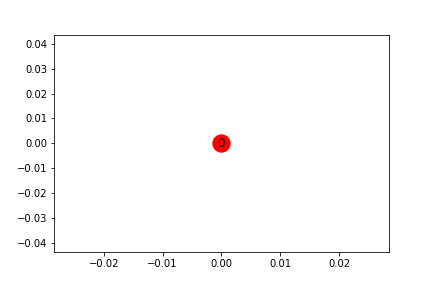
\includegraphics[width=8cm]{grafo_completo_grado_1}
	\caption{Grafo $L_1$}
\end{figure}
\begin{figure}
	\centering
	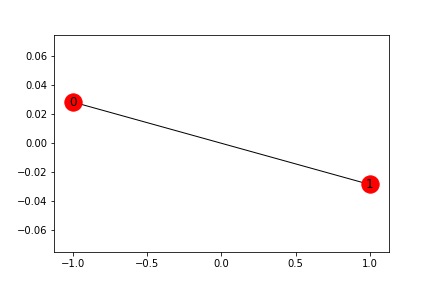
\includegraphics[width=8cm]{grafo_completo_grado_2}
	\caption{Grafo $L_2$}
\end{figure}
\begin{figure}
	\centering
	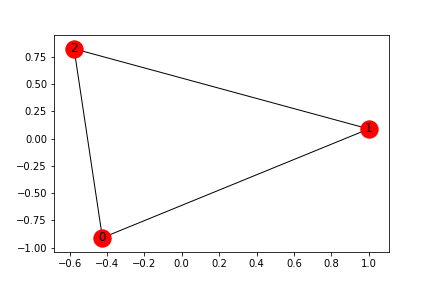
\includegraphics[width=8cm]{grafo_completo_grado_3}
	\caption{Grafo $L_3$}
\end{figure}
\begin{figure}
	\centering
	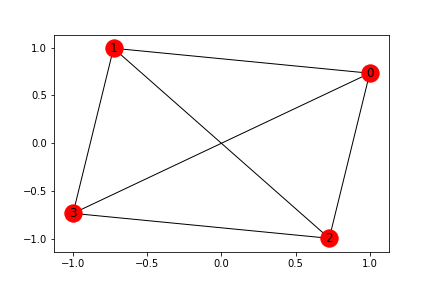
\includegraphics[width=8cm]{grafo_completo_grado_4}
	\caption{Grafo $L_4$}
\end{figure}
\begin{figure}
	\centering
	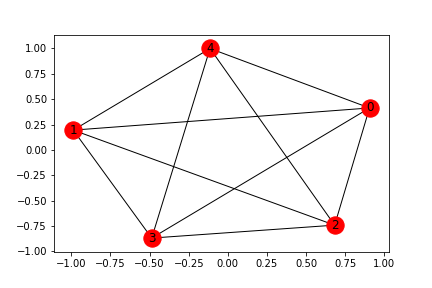
\includegraphics[width=8cm]{grafo_completo_grado_5}
	\caption{Grafo $L_5$}
\end{figure}
\begin{figure}
	\centering
	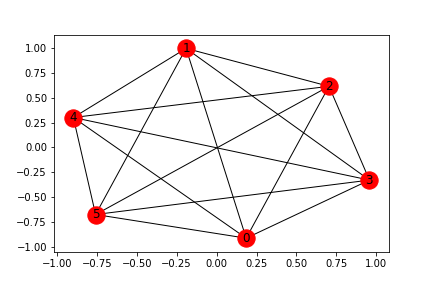
\includegraphics[width=8cm]{grafo_completo_grado_6}
	\caption{Grafo $L_6$}
\end{figure}
\begin{figure}
	\centering
	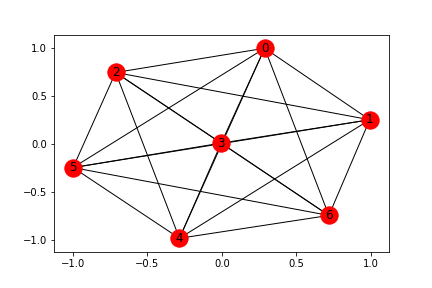
\includegraphics[width=8cm]{grafo_completo_grado_7}
	\caption{Grafo $L_7$}
\end{figure}
\begin{figure}
	\centering
	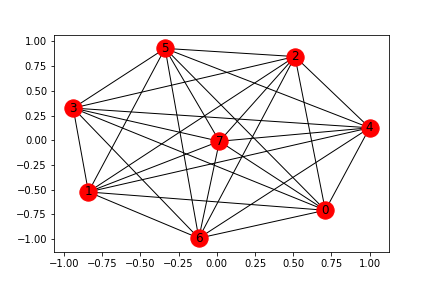
\includegraphics[width=8cm]{grafo_completo_grado_8}
	\caption{Grafo $L_8$}
\end{figure}

\section{Multigrafo}
\subsubsection{\large Calcular la lista de aristas y la matriz de adyacencia para el multigrafo representado en la figura 5}
	Lista de aristas \begin{center}
		\begin{tabular}{ |c|c|c| } 
			\hline
			($n_1,n_2$) \\ 
			($n_2,n_1$) \\ 
			($n_2,n_3$)\\
			($n_2,n_4$)\\
			($n_4,n_4$)\\
			($n_4,n_3$)\\
			($n_3,n_5$)\\
			($n_5,n_4$)\\
			\hline
		\end{tabular}
	\end{center}
Matriz de Adyacencia:
$$\begin{pmatrix}
	0 & 1 & 0 & 0 & 0 \\ 
	1 & 0 & 0 & 0 & 0 \\ 
	0 & 1 & 0 & 1 & 0 \\ 
	0 & 1 & 0 & 1 & 1 \\ 
	0 & 0 & 1 & 0 & 0
\end{pmatrix}$$ 


\section{Grafo pesado}
\subsubsection{\large Calcular la lista de aristas y la matriz de adyacencia del grafo pesado que aparece en la figura 5}

Lista de aristas \begin{center}
	\begin{tabular}{ |c|c|c| } 
		\hline
		($n_1,n_2,5$) \\ 
		($n_2,n_3,1$)\\
		($n_2,n_4,6$)\\
		($n_3,n_5,5$)\\
		($n_4,n_3,3$)\\
		($n_5,n_4,1$)\\
		\hline
	\end{tabular}
\end{center}
Matriz de Adyacencia:
$$\begin{pmatrix}
0 & 0 & 0 & 0 & 0 \\ 
5 & 0 & 0 & 0 & 0 \\ 
0 & 1 & 0 & 0 & 0 \\ 
0 & 6 & 0 & 3 & 1 \\ 
0 & 0 & 5 & 0 & 0
\end{pmatrix}$$ 



\section{Grafo bipartito}
\subsubsection{\large Calcular la matriz de incidencia del grafo bipartito mostrado en el figura 6. Cual sería la matriz de incidencia si no existiera en dicho grafo el nodo m5 ?}


Matriz de Incidencia:
$$\begin{pmatrix}
0 & 1 & 1 & 0 & 0 \\ 
1 & 0 & 0 & 0 & 1 \\ 
0 & 0 & 0 & 0 & 1 \\ 
1 & 0 & 0 & 1 & 0 \\ 
0 & 1 & 0 & 0 & 0
\end{pmatrix}$$ 

Matriz de Incidencia sin nodo $m_5$:
$$\begin{pmatrix}
0 & 1 & 1 & 0  \\ 
1 & 0 & 0 & 0  \\ 
0 & 0 & 0 & 0  \\ 
1 & 0 & 0 & 1  \\ 
0 & 1 & 0 & 0 
\end{pmatrix}$$ 



\section{Grafo proyección 1}
\subsubsection{\large Dibujar el grafo proyección de nodos del grafo bipartito de la figura 6 y demostrar que el grafo proyección de nodos viene descrito por una matriz de adyacencia $P$ tal que $P = BB^T$}

\begin {center}
\begin{tikzpicture}
[scale=.8,auto=left,every node/.style={circle,fill=blue!20}]
\node (n4) at (4,8)  {4};
\node (n5) at (8,9)  {5};
\node (n1) at (11,8) {1};
\node (n2) at (9,6)  {2};
\node (n3) at (5,5)  {3};

\foreach \from/\to in {n1/n5,n2/n4,n2/n3}
\draw (\from) -- (\to);

\end{tikzpicture}
\end{center}

$$P=\begin{pmatrix}
	0 & 1 & 1 & 0 & 0 \\ 
	1 & 0 & 0 & 0 & 1 \\ 
	0 & 0 & 0 & 0 & 1 \\ 
	1 & 0 & 0 & 1 & 0 \\ 
	0 & 1 & 0 & 0 & 0
\end{pmatrix} . \begin{pmatrix}
0 & 1 & 0 & 1 & 0 \\ 
1 & 0 & 0 & 0 & 1 \\ 
1 & 0 & 0 & 0 & 0 \\ 
0 & 0 & 0 & 1 & 0 \\ 
0 & 1 & 1 & 0 & 0
\end{pmatrix}= \begin{pmatrix}
0 & 0 & 0 & 0 & 1 \\ 
0 & 0 & 1 & 1 & 0 \\ 
0 & 1 & 0 & 0 & 0 \\ 
0 & 1 & 0 & 0 & 0 \\ 
1 & 0 & 0 & 0 & 0
\end{pmatrix} $$ 



\subsubsection{\large Dibujar el grafo proyección de grupos del grafo bipartito de la figura 6 y demostrar que el grafo proyección de grupos viene descrito por una matriz de adyacencia $P$ tal que $P = BB^T$}

\begin {center}
\begin{tikzpicture}
[scale=.8,auto=left,every node/.style={circle,fill=blue!20}]
\node (n4) at (4,8)  {4};
\node (n5) at (8,9)  {5};
\node (n1) at (11,8) {1};
\node (n2) at (9,6)  {2};
\node (n3) at (5,5)  {3};

\foreach \from/\to in {n1/n5,n1/n4,n2/n3}
\draw (\from) -- (\to);

\end{tikzpicture}
\end{center}


$$P=\begin{pmatrix}
0 & 1 & 0 & 1 & 0 \\ 
1 & 0 & 0 & 0 & 1 \\ 
1 & 0 & 0 & 0 & 0 \\ 
0 & 0 & 0 & 1 & 0 \\ 
0 & 1 & 1 & 0 & 0
\end{pmatrix}.\begin{pmatrix}
0 & 1 & 1 & 0 & 0 \\ 
1 & 0 & 0 & 0 & 1 \\ 
0 & 0 & 0 & 0 & 1 \\ 
1 & 0 & 0 & 1 & 0 \\ 
0 & 1 & 0 & 0 & 0
\end{pmatrix}= 
\begin{pmatrix}
0 & 0 & 0 & 1 & 1 \\ 
0 & 0 & 1 & 0 & 0 \\ 
0 & 1 & 0 & 0 & 0 \\ 
1 & 0 & 0 & 0 & 0 \\ 
1 & 0 & 0 & 0 & 0
\end{pmatrix} $$ 

\subsubsection{\large En un grafo simple no dirigido $k_i \in [0, N - 1]$, y en un red dirigida $k_i^{in}\in[0, N - 1]$ y $k_i^{out} \in [0, N - 1]$.}
\textit{Ejercicio propuesto en clase}

El resultado es evidente, puesto que en un grafo no dirigido como maximo el nodo puede estar conectado con todos los otros nodos, menos él mismo, lo cual hace que esté en un rango entre 0 ( si no esta conectado a nadie) y N-1 cuando esta conectado a todos los otros nodos.
En los otros casos, el razonamiento es el mismo puesto que se habla de grafos dirigidos y no multigrafos (en los cuales se llegaría hasta N)

\subsubsection{\large Se tiene que para una red simple $L=\frac{1}{2}\langle k\rangle N$}
\textit{Ejercicio propuesto en clase}

Tenemos por definición que: 
$$L=\frac{1}{2}\langle k\rangle N=\frac{1}{2}\frac{1}{N}(\sum_{i=1}^{N}\sum_{j=1}^{N}A_{ij}) N=\frac{1}{2}(\sum_{i=1}^{N}\sum_{j=1}^{N}A_{ij}) $$

donde la ultima igualdad es trivial puesto que en la matriz de adyacencia aparece el numero de aristas repetido dos veces.


\subsubsection{\large Calcular la distribución de probabilidad de grados del grafo no dirigido de la figura 5 y ver que está normalizada}
\begin{itemize}
\item $P(1)=1/5$
\item$P(2)=1/5$
\item $P(3)=3/5$
\end{itemize}
$P(1)+P(2)+P(3)=1$


\subsubsection{\large Calcular la distribución de probabilidad de grados del grafo dirigido y del multigrafo de la figura 5 y ver que está normalizada}
Grafo dirigido:

Saliente
\begin{itemize}
	\item $P(1)=4/5$
	\item$P(2)=1/5$

\end{itemize}
$P(1)+P(2)=1$

Entrante
\begin{itemize}
	\item $P(0)=1/5$
	\item$P(1)=2/5$
	\item $P(2)=2/5$

\end{itemize}
$P(1)+P(2)+P(0)=1$


Multigrafo:

Saliente
\begin{itemize}
	\item $P(1)=3/5$
	\item$P(2)=1/5$
	\item$P(3)=1/5$
\end{itemize}
$P(1)+P(2)+P(3)=1$

Entrante
\begin{itemize}
	\item $P(1)=3/5$
	\item$P(2)=1/5$
	\item $P(3)=1/5$
	
\end{itemize}
$P(1)+P(2)+P(3)=1$

\subsubsection{\large En el grafo no dirigido de la figura 5 calcular el número total de caminos cíclicos de longitud n = 3 que empiezan en los nodos }

$N=Traza\begin{pmatrix}
	0 & 1 & 0 & 0 & 0 \\ 
	1 & 0 & 1 & 1 & 0 \\ 
	0 & 1 & 0 & 1 & 1 \\ 
	0 & 1 & 1 & 0 & 1 \\ 
	0 & 0 & 1 & 1 & 0
	\end{pmatrix}^3=
	Traza\begin{pmatrix}
	0 & 3 & 1 & 1 & 2 \\ 
	3 & 2 & 6 & 6 & 2 \\ 
	1 & 6 & 4 & 5 & 5 \\ 
	1 & 6 & 5 & 4 & 5 \\ 
	2 & 2 & 5 & 5 & 2
	\end{pmatrix}=12$

Si el número nos parece grande, debemos recordar que no hablamos de caminos cíclicos auto evitados.

\subsubsection{\large Demostrar que para una red regular en forma de anillo donde cada nodo tiene grado k = 2m el coeficiente de agrupamiento es $C = 3(m - 1)/2(2m - 1)$}
Sea un grafo con grado $K=2m$

Para calcularlo el coeficiente de agrupamiento solo tenemos que tener en cuenta el numero de triángulos en el grafo de manera que uno de los nodos del triangulo sea nuestro nodo y el numero de tripletas en el grafo.

El numero de tripletas es el mismo que el de posibles links entre nodos vecinos de i, con lo que lo unico que tenemos que calcular es el orden del grafo completo que tuviese "m" links:
$$N_tripletas=\frac{2m(2m-1)}{2}=m(2m-1)$$

Para el numero de triángulos basta ver:

$$N_{triangulos}=3\sum_{j=0}^{m-1}j=3\frac{m(m-1)}{2}$$

Con lo cual, dividiendo por la formula que tenemos en los apuntes:
$$C=\frac{1}{N}\sum_{i=1}^{N}\frac{3(m - 1)}{2(2m - 1)}=\frac{3(m - 1)}{2(2m - 1)}$$

\chapter{Redes de neuronas}
\section{Puertas logicas}
\subsubsection{\large Elaborar las puertas lógicas anteriores mediante una red neuronal de tipo McCulloch-Pitts eligiendo convenientemente los valores de los pesos y de los umbrales} 
Puerta lógica OR:
\begin{center}
\begin{tikzpicture}[scale=.8,auto=left,every node/.style={circle,fill=blue!20}]
\node (n1) at (2,7)  {$I_1$};
\node (n2) at (2,5)  {$I_2$};
\node (n3) at (5,6)  {$\sum$};
\node (n4) at (8,6)  {$f()$};
\node (n5) at (11,6)  {$Y$};

\draw (n1) -- (n3) node [midway,fill=white]{$\omega_1$};
\draw (n2) -- (n3) node [midway,fill=white,below]{$\omega_2$};
\draw (n4) -- (n3);
\draw (n4) -- (n5);

\end{tikzpicture}
\end{center}
Parametros: $\omega_1=1$ y  $\omega_2=1$

Funcion: $$ 
y=\left \{
\begin{array}{rcl}
	1, & \mbox{si } & y \geq 1 \\
	0, & \mbox{si } & y <1
\end{array}
\right .
$$

Puerta lógica AND:
\begin{center}
	\begin{tikzpicture}[scale=.8,auto=left,every node/.style={circle,fill=blue!20}]
	\node (n1) at (2,7)  {$I_1$};
	\node (n2) at (2,5)  {$I_2$};
	\node (n3) at (5,6)  {$\sum$};
	\node (n4) at (8,6)  {$f()$};
	\node (n5) at (11,6)  {$Y$};
	
	\draw (n1) -- (n3) node [midway,fill=white]{$\omega_1$};
	\draw (n2) -- (n3) node [midway,fill=white,below]{$\omega_2$};
	\draw (n4) -- (n3);
	\draw (n4) -- (n5);
	
	\end{tikzpicture}
\end{center}
Parametros: $\omega_1=1$ y  $\omega_2=1$

Funcion: $$ 
y=\left \{
\begin{array}{rcl}
1, & \mbox{si } & y \geq 2 \\
0, & \mbox{si } & y <2
\end{array}
\right .
$$

Puerta lógica NOT:
\begin{center}
	\begin{tikzpicture}[scale=.8,auto=left,every node/.style={circle,fill=blue!20}]
	\node (n1) at (2,7)  {$I_1$};
	\node (n3) at (5,6)  {$\sum$};
	\node (n4) at (8,6)  {$f()$};
	\node (n5) at (11,6)  {$Y$};
	
	\draw (n1) -- (n3) node [midway,fill=white]{$\omega_1$};
	\draw (n4) -- (n3);
	\draw (n4) -- (n5);
	
	\end{tikzpicture}
\end{center}
Parametros: $\omega_1=1$.

Funcion: $$ 
y=\left \{
\begin{array}{rcl}
0, & \mbox{si } & y \geq 1 \\
1, & \mbox{si } & y <1
\end{array}
\right .
$$

Puerta lógica XOR:
\begin{center}
	\begin{tikzpicture}[scale=.8,auto=left,every node/.style={circle,fill=blue!20}]
	\node (n6) at (-1,7)  {$I_1$};
	\node (n7) at (-1,2)  {$I_2$};
	\node (n1) at (2,7)  {$I_3$};
	\node (n2) at (2,2)  {$I_4$};
	\node (n3) at (5,4)  {$\sum$};
	\node (n4) at (8,4)  {$f()$};
	\node (n5) at (11,4)  {$Y$};
	
	\draw (n1) -- (n3) node [midway,fill=white]{$\omega_5$};
	\draw (n2) -- (n3) node [midway,fill=white,below]{$\omega_6$};
	\draw (n4) -- (n3);
	\draw (n4) -- (n5);
		\draw (n6) -- (n1)node [midway,fill=white]{$\omega_1$};
		\draw (n7) -- (n1)node [near end,fill=white]{$\omega_2$};
		\draw (n6) -- (n2)node [near end,fill=white]{$\omega_3$};
		\draw (n7) -- (n2)node [midway,fill=white]{$\omega_4$};
	\end{tikzpicture}
\end{center}
Parametros: $\omega_1=2$,$\omega_2=2$
,$\omega_3=-1$
,$\omega_4=-1$
,$\omega_6=2$
 y  $\omega_5=2$

Funcion: $$ 
y=\left \{
\begin{array}{rcl}
1, & \mbox{si } & y \geq 1 \\
0, & \mbox{si } & y <1
\end{array}
\right .
$$
\section{Hodgkin-Huxley}
\subsubsection{\large Simular el modelo de Hodgkin-Huxley y determinar el rango de I en el que aparecen oscilaciones} 
El modelo de Hodgkin y Huxley describe cómo se inician y transmiten los potenciales de acción en las neuronas. Consiste en un conjunto de ecuaciones diferenciales ordinarias no lineales que aproxima las características eléctricas de células excitables, en nuestro caso, las neuronas.


 $$I = C_m\frac{{\mathrm d} V_m}{{\mathrm d} t}  + \bar{g}_\text{K}n^4(V_m - V_K) + \bar{g}_\text{Na}m^3h(V_m - V_{Na}) + \bar{g}_l(V_m - V_l),$$

 $$\frac{dn}{dt} = \alpha_n(V_m)(1 - n) - \beta_n(V_m) n$$

 $$\frac{dm}{dt} = \alpha_m(V_m)(1 - m)  - \beta_m(V_m) m$$

 $$\frac{dh}{dt} = \alpha_h(V_m)(1 - h) - \beta_h(V_m) h$$

donde ''I'' es la corriente por unidad de area, y $\alpha_i $ and $\beta_i $ son las ratios de los canales de iones que no depende del tiempo. $\bar{g}_n$ es el valor máximo de la conductancia. '' n '', '' m '' y '' h '' son cantidades adimensionales entre 0 y 1 que están asociadas con la activación del canal de potasio, la activación del canal de sodio y la inactivación del canal de sodio, respectivamente. 

He concentrado en un grafico \ref{h} la resolucion del ejercicio, de manera que se puede observar los rangos de I que producen actividad con un grafico superpuesto. 
\begin{figure}
	\centering
	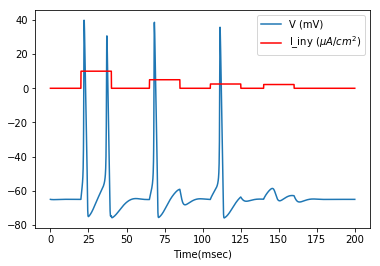
\includegraphics[width=12cm]{hodgkin}
	\caption{Representacion del modelo HH con la corriente}
	\label{h}
\end{figure}

\section{Modelo FN}

\subsubsection{\large Integrar numéricamente el modelo de FN y estudiar comportamientos dinámicos que pueden aparecer} 


El modelo de FitzHugh-Nagumo (FHN) describe un prototipo de un sistema excitable (por ejemplo, una neurona). Toma su nombre de Richard FitzHugh (1922 - 2007), quien propuso el modelo teórico en 1961, así como de J. Nagumo y otros, que construyeron un circuito electrónico equivalente.

$$
 \dot{v}=v-\frac{v^3}{3} - u + I_{\rm ext} 
 $$
 
 $$
 \tau \dot{u} = v+a-b u
 $$

Para mostrar los distintos tipos de comportamientos se han creado una serie de graficas que los exhiben: \ref{1fn}\ref{2fn}\ref{3fn}\ref{4fn}.

\begin{figure}
	\centering
	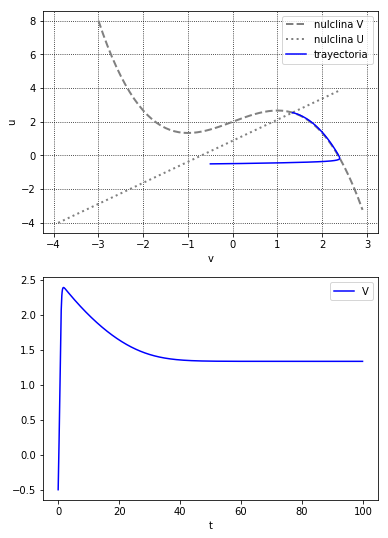
\includegraphics[width=9cm]{2}
	\caption{Tendencia al punto estable}
	\label{1fn}
\end{figure}

\begin{figure}
	\centering
	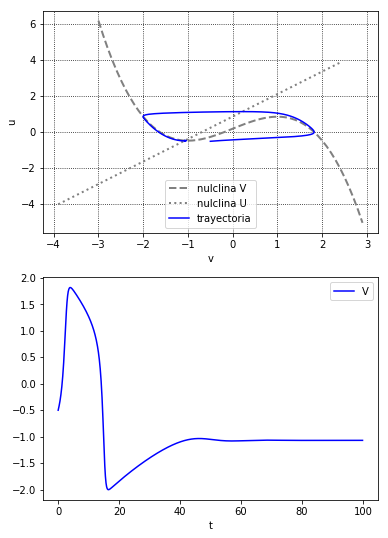
\includegraphics[width=9cm]{0-2}
	\caption{Tendencia al punto estable}
	\label{2fn}
\end{figure}

\begin{figure}
	\centering
	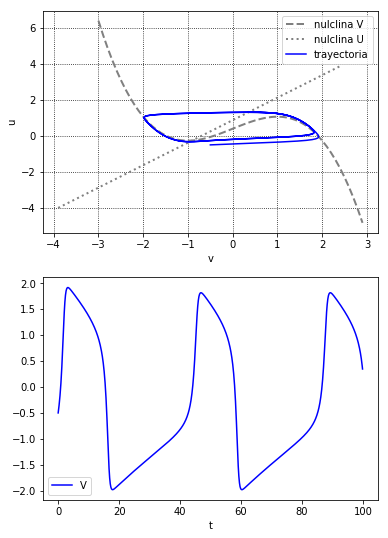
\includegraphics[width=9cm]{0-4}
	\caption{Si recibe suficiente fuerza, empiezan comportamientos periodicos}
	\label{3fn}
\end{figure}

\begin{figure}
	\centering
	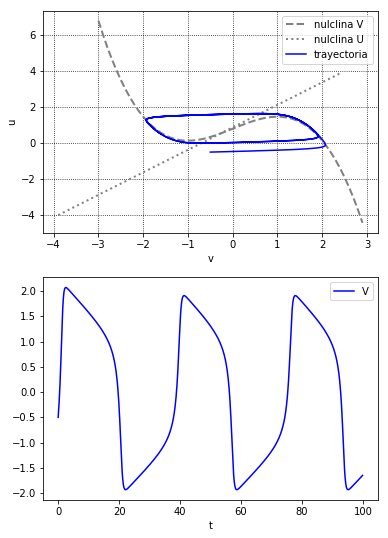
\includegraphics[width=9cm]{0-6}
	\caption{Comportamiento periodico}
	\label{4fn}
\end{figure}

\section{Modelo Tsodyks-Markram}

\subsubsection{\large Simular el modelo de Tsodyks-Markram de sinapsis dinámica y ver la forma del potencial postsináptico excitador EPSP usando por ejemplo un modelo lineal de integración y disparo para la neurona postsináptica cuando está sometida a un tren de pulsos presinápticos periódicos que llegan a una frecuencia f dada} 
Se puede consultar el script del intento en el apéndice 3, sin embargo, no ha dado resultados creíbles.











\chapter{Redes sociales}

\section{Modelo del votante Barabasi-Albert y S-M}

\subsubsection{\large Simular el modelo del votante en una red pequeño mundo y en una red de Barabási-Albert y estudiar su comportamiento emergente} 
El modelo de votante es un modelo de no equilibrio que tiene solucion analitica en cualquier dimension. Tendriamos N agentes sociales, nodos de una red. Cada agente puede estar en dos estados ($\pm1$). Cada paso temporal es elegido un agente y uno de sus vecinos y adquieren el mismo estado.

Red de pequeño mundo:

En la figura se puede ver el aspecto de nuestra red \ref{1} (se ha creado segun los estándares, pero el output de python es bastante reducido). El aspecto final \ref{2}. Y la fraccion a lo largo del tiempo, propia de estos sistemas complejos: \ref{3}.
\begin{figure}
	\centering
	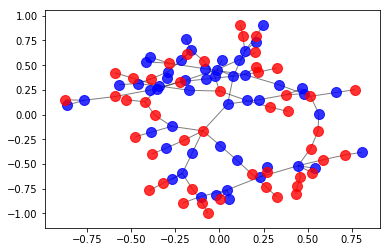
\includegraphics[width=9cm]{dist_inic_small}
	\caption{Estado inicial para red pequeño mundo}
	\label{1}
\end{figure}

\begin{figure}
	\centering
	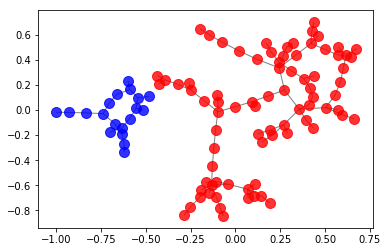
\includegraphics[width=9cm]{final_small}
	\caption{Estado final (Se representa distinto para observar mejor la clusterizacion)}
	\label{2}
\end{figure}

\begin{figure}
	\centering
	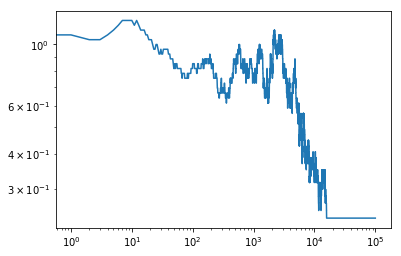
\includegraphics[width=9cm]{frac_small}
	\caption{Fracción de pares con distinta opinión en función del tiempo en un modelo del votante}
	\label{3}
\end{figure}

Red de Barabási-Albert:

En la figura se puede ver el aspecto de nuestra red \ref{4} (se ha creado segun los estándares, pero el output de python es bastante reducido). El aspecto final\ref{5}. Y la fraccion a lo largo del tiempo, propia de estos sistemas complejos: \ref{6}.
En este caso vemos algunas incoherencias, pero son comprensibles debido al bajo numero de nodos de nuestra red (por limitaciones de mi ordenador).
\begin{figure}
	\centering
	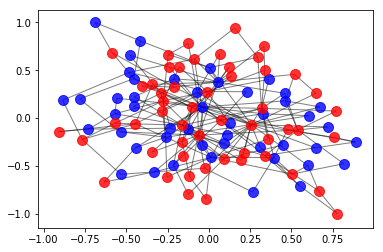
\includegraphics[width=9cm]{barra_inic}
	\caption{Estado inicial para red pequeño mundo}
	\label{4}
\end{figure}

\begin{figure}
	\centering
	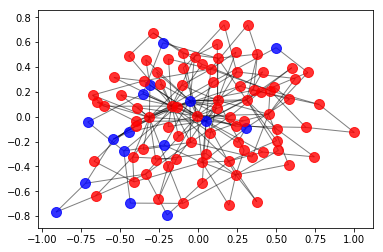
\includegraphics[width=9cm]{barra_fin}
	\caption{Estado final}
	\label{5}
\end{figure}

\begin{figure}
	\centering
	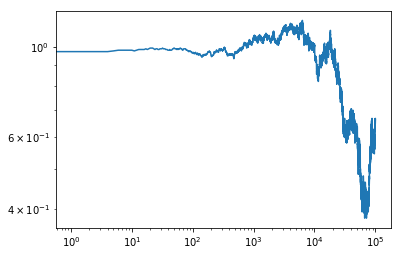
\includegraphics[width=9cm]{barra_frac}
	\caption{Fracción de pares con distinta opinión en función del tiempo en un modelo del votante}
	\label{6}
\end{figure}

\section{Competicion de lenguas}
\subsubsection{\large Estudiar las soluciones del sistema anterior y su estabilidad e interpretar cada uno de los estados estacionarios posibles.} 

Estamos ante el estudio del sistema de competición de lenguas, que viene dictaminado por la ecuación:
$$dm_A/dt=s(m_A)^a(1-m_A)-(1-s)(1-m_A)^am_A$$
Esta ecuacion tiene 3 puntos de equilibrio para $a\neq1$:
Si $a>1$ tenemos $m_A=0$ y $m_A=1$ como puntos de equilibro estables, aquellos en los que alguna otra lengua elimina a la competencia. Tenemos otro punto critico entre 0 y 1 que representa un estado inestable de equilibrio entre las lenguas.

Para $a<1$ el problema es el mismo pero la cualidad de estabilidad se invierte en los puntos criticos encontrados.
(Se ha consultado para este apartado el articulo \textit{Microscopic Abrams-Strogatz model of language competition})




\appendix
\chapter{Tema 1: Códigos}

\section{Atractores de Lorentz y Rossler}

Atractor de Lorentz
\lstinputlisting[language=Python]{tema1/lorenz.py}

Atractor de Rossler
\lstinputlisting[language=Python]{tema1/rossler.py}

\section{Autómatas celulares }

Juego de la vida 
\lstinputlisting[language=Python]{tema1/game_of_life_2.py}

Buscador para el juego de la vida
\lstinputlisting[language=Python]{tema1/game_of_life_searcher.py}

Pila de arena
\lstinputlisting[language=Python]{tema1/sand_pile.py}

Hormiga de langton
\lstinputlisting[language=Python]{tema1/ants.py}

\chapter{Tema 2: Códigos}

\section{Grafos completos}

\lstinputlisting[language=Python]{tema2/complete_graph_generator.py}

\chapter{Tema 3: Códigos}

\section{Hodgkin–Huxley modelo}
\lstinputlisting[language=Python]{tema4/Hodgkin_huxley.py}


\section{FitzHugh–Nagumo modelo}
\lstinputlisting[language=Python]{tema4/Final_f_N.py}

\section{Tsodyks-Markram modelo}
\lstinputlisting[language=Python]{tema4/stodysk.py}
\chapter{Tema 4: Códigos}

\section{Voter model con Barabasi-Albert}
\lstinputlisting[language=Python]{tema6/voter_model.py}

\section{Voter model con Small-World}
\lstinputlisting[language=Python]{tema6/small_world.py}



\end{document}



\begin{document}
	


\title{\LARGE {\bf Ejercicios de Redes complejas en fisica y neurociencia}\\
 \vspace*{6mm}
}

\author{Bartolomé Ortiz Viso}
\submitdate{Mayo 2018}

\narrowlinespacing
\maketitle

\preface

\addcontentsline{toc}{chapter}{Abstract}

\begin{abstract}

Este trabajo compone la resolucion de algunos de los ejercicios propuestos en la asignatura del Master de Fisica y Matematicas fisymat de la Universidad de Granada denominada Fisica de redes complejas. La primera parte de la asignatura es impartida por el profesor Joaquín Torres. 

Generalmente la mayoría de los ejercicios poseen algún componente computacional, ya sean cálculos, simulación o visualización. Con el fin de resaltar la importancia de este aspecto, pero no dificultar la lectura, los códigos están adjuntos y se pueden consultar en los apéndices dejando solo para el grueso del texto las conclusiones derivadas y las visualizaciones. 

Así mismo muchos de los códigos empleados tambien poseen un salida visual en forma de animaciones y videos que puede ser interesante observar. Para este fin puede consultar el respositorio en github donde están todos los códigos utilizados, las salidas de los mismos y por supuesto, una versión de este documento en pdf y latex bajo la licencia creative commons:

\url{http://www.github.com/thebooort/Complex-Networks-and-Neuroscience}
 
 Algunos de los códigos utilizados utilizan partes de otras librerías o códigos. En esos casos quedan citados los otros responsables y la licencia se adhiere a la que pusieran sus creadores iniciales antes de mis modificaciones para este trabajo.
 

\end{abstract}



\body
\chapter{Sistemas complejos}
\section{Atractores}
\subsubsection{\large Simular y analizar el comportamiento complejo del atrayente de Lorenz} 
El descubrimiento de este atractor data de 1963, cuando Edward Norton Lorenz desarrolló un modelo matemático simplificado para la convección atmosférica. El modelo es un sistema de ecuaciones diferenciales ordinarias compuesto por tres ecuaciones ahora conocidas como las ecuaciones de Lorenz:
$$\left\{\begin{matrix}\frac{\mathrm{d}x}{\mathrm{d}t} &= \sigma (y - x), \\
	\frac{\mathrm{d}y}{\mathrm{d}t} &= x (\rho - z) - y, \\
	\frac{\mathrm{d}z}{\mathrm{d}t} &= x y - \beta z.\end{matrix}\right.$$
Normalmente se asume que los parametros $\sigma$, $\rho$, y $\beta$ son positivos. El interés en este modelo proviene de que para una seleccion de valores como $\sigma = 10$, $\beta = 8/3$ and $\rho = 28 $ el sistema exhibe un comportamiento caótico.

Si $\rho < 1$ entonces sólo hay un punto de equilibrio en el origen. Este punto además es un atractor global.

Si $\rho = 1$ entonces la en nuestra dinámica aparece una bifurcacion de pitchfork , y para  $\rho > 1 $ apareceen dos puntos de equilibrio, a saber $\left( \sqrt{\beta(\rho-1)}, \sqrt{\beta(\rho-1)}, \rho-1 \right) $ and $\left( -\sqrt{\beta(\rho-1)}, -\sqrt{\beta(\rho-1)}, \rho-1 \right). $ 
Este par de puntos será estable si : $\rho < \sigma\frac{\sigma+\beta+3}{\sigma-\beta-1}$

Como avanzábamos para valores como $\rho = 28$, $\sigma = 10$, and $\beta = 8/3$, el sistema de Lorenz tiene soluciones caóticas (es decir que, aunque no todas las soluciones son caóticas algunas de ellas si pueden presentar este comportamiento).

 Casi todos los puntos iniciales tenderán a un conjunto invariable que es lo que denominamos el atractor de Lorenz (véase figura:\ref{lorentz1}), cuya forma geométrica es reconocible. Este comportamiento caótico se refleja en la gran sensibilidad del atractor frente a cambios en las condiciones iniciales como se puede ver en la grafica \ref{lorentz2}.\textit{ Las graficas pertenecen a extractos de animaciones que pueden consultarse en github.}
 
 \begin{figure}
 	\centering
 	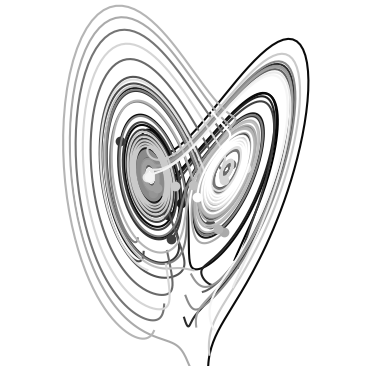
\includegraphics[width=8cm]{lorentz}
 	\caption{Atractor de Lorentz}
 	\label{lorentz1}
 \end{figure}
 \begin{figure}
 	\centering
 	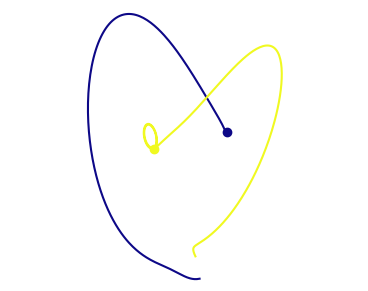
\includegraphics[width=8cm]{lorentz1}
 	\caption{Atractor de Lorentz: variacion respecto a condiciones iniciales}
 	\label{lorentz2}
 \end{figure}
 
 \subsubsection{\large Simular y analizar el comportamiento complejo del atrayente de Rossler} 
 
 El atractor de Rössler es el atractor del sistema de Rössler, un sistema de tres ecuaciones diferenciales ordinarias no lineales estudiadas por Otto E. Rössler. Estas ecuaciones diferenciales definen un sistema dinámico del tiempo-continuo que muestra dinámicas caóticas asociadas con las propiedades fractales del atractor:
 $$\left\{\begin{matrix}\frac{dx}{dt} &= -y - z \\
 \frac{dy}{dt} &= x + ay, \\
 \frac{dz}{dt} &= b + z(x-c).\end{matrix}\right.$$
 Rössler estudió el atractor caótico con $ a = 0.2 $, $ b = 0.2 $ y $ c = 5.7 $, aunque las propiedades de $ a = 0.1 $, $ b = 0.1 $, y $ c = 14 $ han sido más comúnmente utilizadas desde entonces.
 De nuevo con estos parámetros podemos encontrar orbitas con comportamiento caótico como se representa en la figura \ref{rossler1}. \textit{ La grafica pertenecen a extractos de animaciones que pueden consultarse en github.}
  \begin{figure}
  	\centering
  	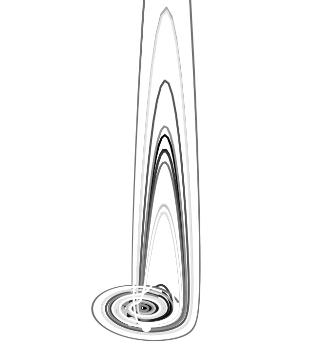
\includegraphics[width=8cm]{rossler}
  	\caption{Atractor de Rossler}
  	\label{rossler1}
  \end{figure}
  
 \section{Juego de la vida}
 \subsubsection{\large Simular el juego de la vida y estudiar su comportamiento emergente} 
  
  El juego de la vida es un autómata celular diseñado por el matemático británico John Horton Conway en 1970.
  
  Hizo su primera aparición pública en el número de octubre de 1970 de la revista Scientific American, en la columna de juegos matemáticos de Martin Gardner. Desde un punto de vista teórico, es interesante porque es equivalente a una máquina universal de Turing, es decir, todo lo que se puede computar algorítmicamente se puede computar en el juego de la vida.
    \begin{figure}
    	\centering
    	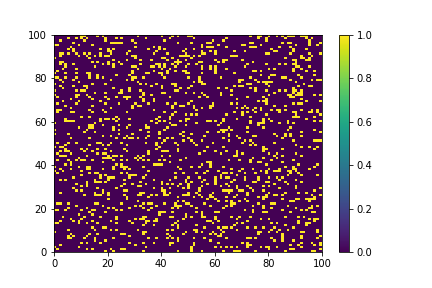
\includegraphics[width=8cm]{generation0}
    	\caption{Disposicion inicial: partimos de una distribucion aleatoria de puntos en una malla}
    	\label{gol1}
    \end{figure}
  \begin{figure}
  	\centering
  	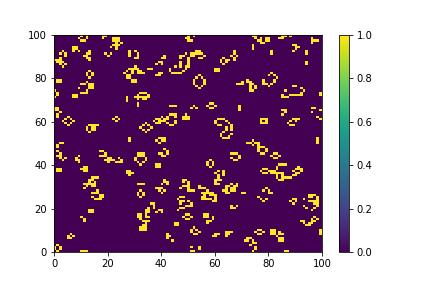
\includegraphics[width=8cm]{generation5}
  	\caption{Evolucion del juego de la vida tras 5 pasos temporale}
  	\label{gol2}
  \end{figure}
  \begin{figure}
  	\centering
  	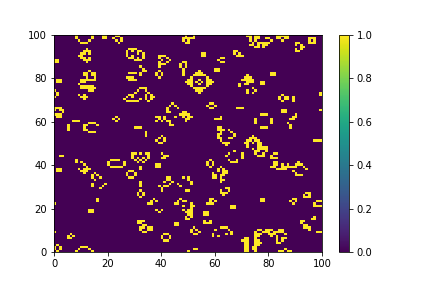
\includegraphics[width=8cm]{generation10}
  	\caption{Evolucion del juego de la vida tras 10 pasos temporales }
  	\label{gol3}
  \end{figure}
  Para profundizar un poco más en el trabajo se ha desarrollado un programa para detectar si patrones implementados generan naves espaciales.
  Las naves espaciales son patrones que reaparecen en otra posición tras completar su período. Esto es, son patrones que tras un número finito de generaciones vuelven a su estado original pero en una ubicación diferente.
  En este caso se han utilizado las reglas estándar. Tras 4 pasos temporales se localizó que la figura era una nave espacial (figuras \ref{gol4} y \ref{gol5})
   \begin{figure}
   	\centering
   	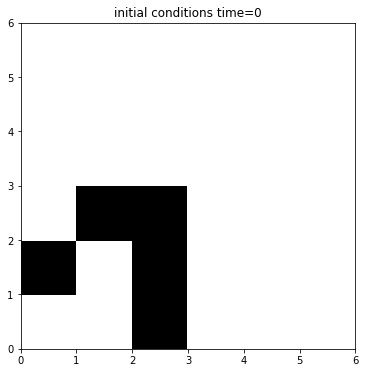
\includegraphics[width=8cm]{searcher_1}
   	\caption{Disposicion inicial encontrada como buena }
   	\label{gol4}
   \end{figure}
    \begin{figure}
    	\centering
    	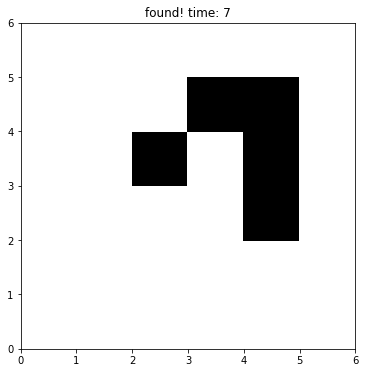
\includegraphics[width=8cm]{searcher_2}
    	\caption{Identidad identica transportadad tras 4 pasos temporales }
    	\label{gol5}
    \end{figure}
    Esta es la nave espacial más famosa, conocida como glider.
\subsubsection{\large Modelo pilas de arena}     
El modelo de pilas de arena es un modelo matemático diseñado para analizar y explicar el comportamiento de autoorganización crítica a través de la teoría de grafos y la teoría de autómatas celulares utilizando herramientas algebraicas.

Si consideramos un plano con una gran cantidad de arena al que se le va añadiendo un poco cada paso temporal, si la pendiente es muy alta, la arena tenderá a caer provocando una avalancha, pues es un estado insetable. Esto se poducirá hasta que todo llegue a un estado estable en cuanto a la pendiente.

Se pueden ver el resultado de las simulaciones en \ref{sand1},\ref{sand2},\ref{sand3}

 \begin{figure}
 	\centering
 	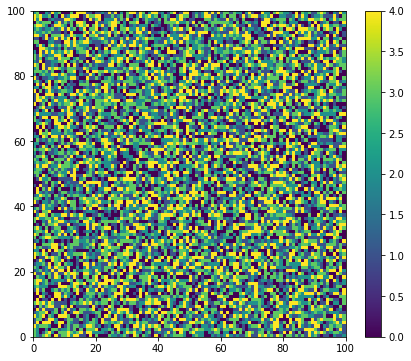
\includegraphics[width=8cm]{pila_arena_random}
 	\caption{Pila de arena con condiciones iniciales aleatorias  }
 	\label{sand1}
 \end{figure}
  \begin{figure}
  	\centering
  	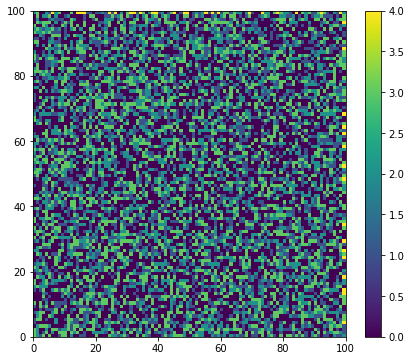
\includegraphics[width=8cm]{pila_arena_random_2}
  	\caption{Sin adicion y partiendo de \ref{sand1} vemos como el sistema tiene a producir avalanchas hasta nivelarse }
  	\label{sand2}
  \end{figure}

 \begin{figure}
 	\centering
 	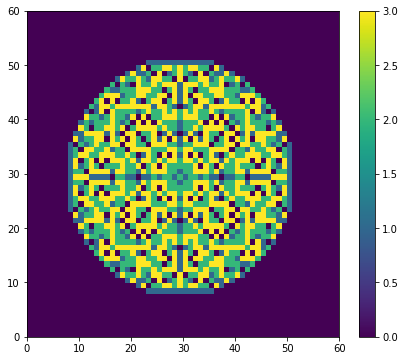
\includegraphics[width=8cm]{pila_arena}
 	\caption{Creacion de fractales cuando añadimos un goteo de arena en el centro durante 100 pasos de tiempo }
 	\label{sand3}
 \end{figure}


    
\subsubsection{\large Modelo hormiga de langton}    
Aunque no partía como ejercicio, buscando información sobre algunas de turing y el juego de la vida también he encontrado otra sencilla maquina con comportamientos emergentes que dejo a continuación.
La hormiga de Langton es un una máquina de Turing bidimensional con un conjunto de reglas muy sencillo, que sin embargo da lugar a comportamientos emergentes complejos.
 La hormiga de Langton clásica opera sobre una rejilla espacial cuadrada, en que cada celda puede estar en uno de dos estados (blanca o negra, 1 o 0, viva o muerta, etc). Fue inventada por Chris Langton en 1986 y su universalidad se demostró en el año 2000.
 
 La hormiga siempre está mirando en una de las cuatro direcciones cardinales y se mueve un cuadrado cada vez, de acuerdo con las siguientes reglas:
 \begin{itemize}
 	\item Si está sobre un cuadrado blanco, cambia el color del cuadrado, gira noventa grados a la izquierda y avanza un cuadrado.
 	\item Si está sobre un cuadrado negro, cambia el color del cuadrado, gira noventa grados a la derecha y avanza un cuadrado.
 \end{itemize}
 
   \begin{figure}
   	\centering
   	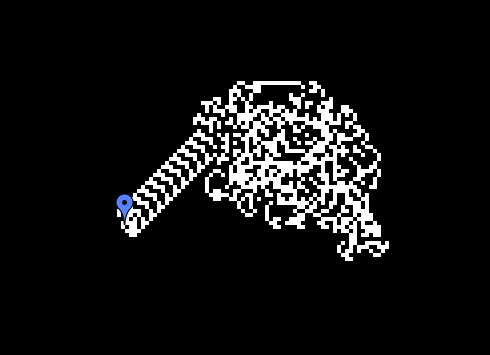
\includegraphics[width=8cm]{ant}
   	\caption{Hormiga tras 11000 pasos temporales. Las condiciones iniciales son nulas salvo la casilla de la hormiga }
   	\label{ant}
   \end{figure}
  



\section{Dimensiones de Haussdorf: variedades continuas y fractales}
\subsubsection{\large Demostrar que con la definición de dimension de Haussdorf se tiene (para variedades continuas:curva, superficie, y volumen) las dimensiones esperadas.} 

Partimos de la formula descrita en los apuntes, la dimension de Haussdorf ($D$) de una variedad viene determinada por:
\begin{equation}
D=\lim_{a\rightarrow 0}(\frac{-ln(N(a))}{ln(a)})
\end{equation}
donde $N(a)$ es el número mínimo de $esferas$ $d–dimensionales$ necesarias para cubrir por completo la variedad en cuestión.
Teniendo en cuenta que $d T \leq D \leq d$, donde $d$ es la dinemsion euclídea y $d_T$ e sla dimension topológica, sabemos de antemano que como todas nuestras variedades son continuas, el valor será $1,2,3$ para la curva, la superficie y le columen, respectivamente. Analizamos caso por caso: 
\begin{itemize}
	\item Curva continua:
	
	En este caso las $esferas$ $d–dimensionales$ son segmentos de longitud $2a$, por tanto, sea una curva continua con longitud $1$:
	\begin{equation}
	\begin{split}
	D=\lim_{a\rightarrow 0}(\frac{-ln(N(a))}{ln(a)})
	&=-\lim_{a\rightarrow 0}(\frac{ln(1/2a)}{ln(a)})\\
	=-\lim_{a\rightarrow 0}(\frac{\frac{d}{da}ln(1/2a)}{\frac{d}{da}ln(a)})
	&=-\lim_{a\rightarrow 0}(\frac{-1/x}{1/x})=1
	\end{split}
	\end{equation}
	\item Superficie continua:
	
	En este caso las $esferas$ $d–dimensionales$ son discos de radio $a$, por tanto, dada una superficie, podemos recubir su borde colocando esferas que abarcan una longitud de $2a$ a lo alto y a lo largo:
	
	\begin{equation}
	\begin{split}
	D=\lim_{a\rightarrow 0}(\frac{-ln(N(a))}{ln(a)})
	&=-\lim_{a\rightarrow 0}(\frac{ln(1/(2a)^2)}{ln(a)})\\
	=-\lim_{a\rightarrow 0}(\frac{\frac{d}{da}ln(1/4x^2)}{\frac{d}{da}ln(a)})
	&=-\lim_{a\rightarrow 0}(\frac{-2/x}{1/x})=2
	\end{split}
	\end{equation}
	
	\item Volumen continuo:
	
	En este caso las $esferas$ $d–dimensionales$ son esferas de radio $2a$, por tanto, dado un volumen continuo podemos recubir su borde colocando esferas que abarcan una longitud de $2a$ a lo alto, a lo ancho y a lo largo :
	\begin{equation}
	\begin{split}
	D=\lim_{a\rightarrow 0}(\frac{-ln(N(a))}{ln(a)})
	&=-\lim_{a\rightarrow 0}(\frac{ln(1/(2a)^3)}{ln(a)})\\
	=-\lim_{a\rightarrow 0}(\frac{\frac{d}{da}ln(1/8x^3)}{\frac{d}{da}ln(a)})
	&=-\lim_{a\rightarrow 0}(\frac{-3/x}{1/x})=3
	\end{split}
	\end{equation}
\end{itemize}


\subsubsection{\large Calcular la dimensión Hausdorff de los siguientes fractales: Conjunto de Cantor, la Isla de Koch, la Alfombra de Sierpinsky y la triangulo de Sierpinsky} 
 Atendiendo a la definición de las notas, tenemos que $$M\sim R^D$$
 donde D es la dimensión fractal. 
 Por tanto si desarrollamos obtenemos: 
$$D=\frac{log(M)}{log(R)}$$
Pasemos a analizar cada uno de los casos. 
\begin{itemize}
	\item Conjunto de cantor:
	
	en este caso tenemos una variedad de masa 1, de manera que en cada paso obtenemos dos subvariedades, estas subvariedades coinciden con la original si aumentamos la escala 3 unidades de la que tenemos, por tanto:  $$D=\frac{log(2)}{log(3)}$$
	
	\item Isla de Koch:
	
	en este caso tenemos una variedad cuya dimension D debe ser $1<D<2$. En esta figura si aplicamos un factor de multiplicacion 3 obtenemos 4 veces la seccion inicial que habíamos aumentado, por tanto:  $$D=\frac{log(4)}{log(3)}$$

	\item Alfombra de Sierpinsky:
	
	en este caso tenemos una variedad cuya dimension D debe ser $1<D<2$. Si aumentamos la figura por un factor 3, obtenemos 8 subvariedades identicas a la original , por tanto:  $$D=\frac{log(8)}{log(3)}$$
	
	\item triangulo de Sierpinsky:
	
	en este caso tenemos una variedad cuya dimension D debe ser $1<D<2$. Si aumentamos la figura por un factor 2, obtenemos 3 subvariedades identicas a la original , por tanto:  $$D=\frac{log(3)}{log(2)}$$
\end{itemize}






\chapter{Redes complejas}
\section{Grafos completos}
\subsubsection{\large Dibuja $L_i$, $i=1,...,8$} 
A continuación se muestran todos los grafos generados a partir del script del anexo.
\begin{figure}
	\centering
	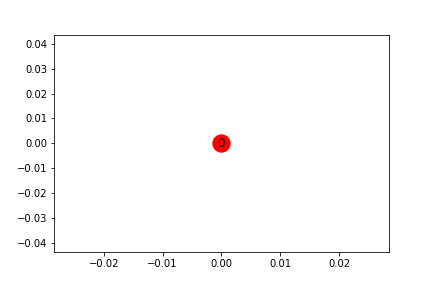
\includegraphics[width=8cm]{grafo_completo_grado_1}
	\caption{Grafo $L_1$}
\end{figure}
\begin{figure}
	\centering
	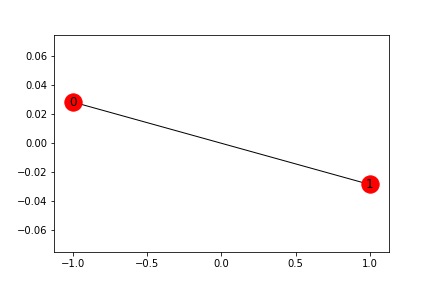
\includegraphics[width=8cm]{grafo_completo_grado_2}
	\caption{Grafo $L_2$}
\end{figure}
\begin{figure}
	\centering
	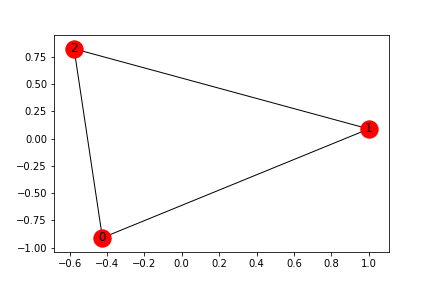
\includegraphics[width=8cm]{grafo_completo_grado_3}
	\caption{Grafo $L_3$}
\end{figure}
\begin{figure}
	\centering
	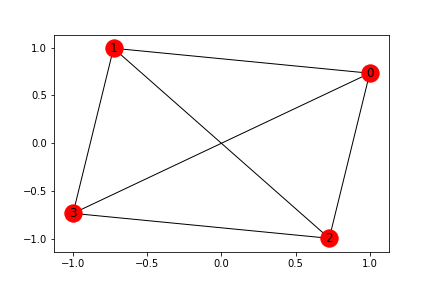
\includegraphics[width=8cm]{grafo_completo_grado_4}
	\caption{Grafo $L_4$}
\end{figure}
\begin{figure}
	\centering
	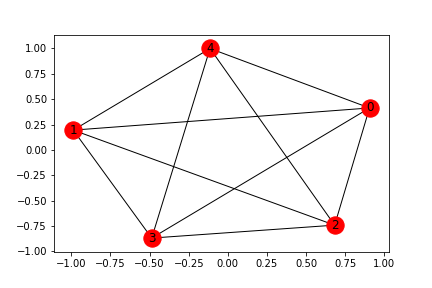
\includegraphics[width=8cm]{grafo_completo_grado_5}
	\caption{Grafo $L_5$}
\end{figure}
\begin{figure}
	\centering
	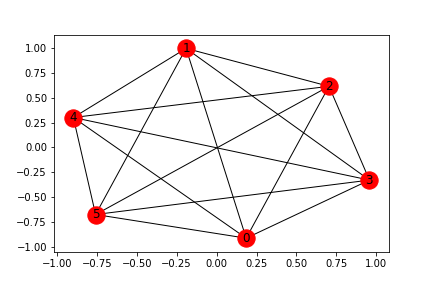
\includegraphics[width=8cm]{grafo_completo_grado_6}
	\caption{Grafo $L_6$}
\end{figure}
\begin{figure}
	\centering
	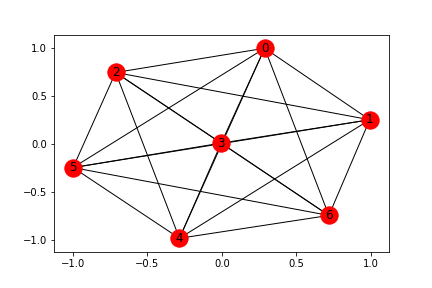
\includegraphics[width=8cm]{grafo_completo_grado_7}
	\caption{Grafo $L_7$}
\end{figure}
\begin{figure}
	\centering
	\includegraphics[width=8cm]{grafo_completo_grado_8}
	\caption{Grafo $L_8$}
\end{figure}

\section{Multigrafo}
\subsubsection{\large Calcular la lista de aristas y la matriz de adyacencia para el multigrafo representado en la figura 5}
	Lista de aristas \begin{center}
		\begin{tabular}{ |c|c|c| } 
			\hline
			($n_1,n_2$) \\ 
			($n_2,n_1$) \\ 
			($n_2,n_3$)\\
			($n_2,n_4$)\\
			($n_4,n_4$)\\
			($n_4,n_3$)\\
			($n_3,n_5$)\\
			($n_5,n_4$)\\
			\hline
		\end{tabular}
	\end{center}
Matriz de Adyacencia:
$$\begin{pmatrix}
	0 & 1 & 0 & 0 & 0 \\ 
	1 & 0 & 0 & 0 & 0 \\ 
	0 & 1 & 0 & 1 & 0 \\ 
	0 & 1 & 0 & 1 & 1 \\ 
	0 & 0 & 1 & 0 & 0
\end{pmatrix}$$ 


\section{Grafo pesado}
\subsubsection{\large Calcular la lista de aristas y la matriz de adyacencia del grafo pesado que aparece en la figura 5}

Lista de aristas \begin{center}
	\begin{tabular}{ |c|c|c| } 
		\hline
		($n_1,n_2,5$) \\ 
		($n_2,n_3,1$)\\
		($n_2,n_4,6$)\\
		($n_3,n_5,5$)\\
		($n_4,n_3,3$)\\
		($n_5,n_4,1$)\\
		\hline
	\end{tabular}
\end{center}
Matriz de Adyacencia:
$$\begin{pmatrix}
0 & 0 & 0 & 0 & 0 \\ 
5 & 0 & 0 & 0 & 0 \\ 
0 & 1 & 0 & 0 & 0 \\ 
0 & 6 & 0 & 3 & 1 \\ 
0 & 0 & 5 & 0 & 0
\end{pmatrix}$$ 



\section{Grafo bipartito}
\subsubsection{\large Calcular la matriz de incidencia del grafo bipartito mostrado en el figura 6. Cual sería la matriz de incidencia si no existiera en dicho grafo el nodo m5 ?}


Matriz de Incidencia:
$$\begin{pmatrix}
0 & 1 & 1 & 0 & 0 \\ 
1 & 0 & 0 & 0 & 1 \\ 
0 & 0 & 0 & 0 & 1 \\ 
1 & 0 & 0 & 1 & 0 \\ 
0 & 1 & 0 & 0 & 0
\end{pmatrix}$$ 

Matriz de Incidencia sin nodo $m_5$:
$$\begin{pmatrix}
0 & 1 & 1 & 0  \\ 
1 & 0 & 0 & 0  \\ 
0 & 0 & 0 & 0  \\ 
1 & 0 & 0 & 1  \\ 
0 & 1 & 0 & 0 
\end{pmatrix}$$ 



\section{Grafo proyección 1}
\subsubsection{\large Dibujar el grafo proyección de nodos del grafo bipartito de la figura 6 y demostrar que el grafo proyección de nodos viene descrito por una matriz de adyacencia $P$ tal que $P = BB^T$}

\begin {center}
\begin{tikzpicture}
[scale=.8,auto=left,every node/.style={circle,fill=blue!20}]
\node (n4) at (4,8)  {4};
\node (n5) at (8,9)  {5};
\node (n1) at (11,8) {1};
\node (n2) at (9,6)  {2};
\node (n3) at (5,5)  {3};

\foreach \from/\to in {n1/n5,n2/n4,n2/n3}
\draw (\from) -- (\to);

\end{tikzpicture}
\end{center}

$$P=\begin{pmatrix}
	0 & 1 & 1 & 0 & 0 \\ 
	1 & 0 & 0 & 0 & 1 \\ 
	0 & 0 & 0 & 0 & 1 \\ 
	1 & 0 & 0 & 1 & 0 \\ 
	0 & 1 & 0 & 0 & 0
\end{pmatrix} . \begin{pmatrix}
0 & 1 & 0 & 1 & 0 \\ 
1 & 0 & 0 & 0 & 1 \\ 
1 & 0 & 0 & 0 & 0 \\ 
0 & 0 & 0 & 1 & 0 \\ 
0 & 1 & 1 & 0 & 0
\end{pmatrix}= \begin{pmatrix}
0 & 0 & 0 & 0 & 1 \\ 
0 & 0 & 1 & 1 & 0 \\ 
0 & 1 & 0 & 0 & 0 \\ 
0 & 1 & 0 & 0 & 0 \\ 
1 & 0 & 0 & 0 & 0
\end{pmatrix} $$ 



\subsubsection{\large Dibujar el grafo proyección de grupos del grafo bipartito de la figura 6 y demostrar que el grafo proyección de grupos viene descrito por una matriz de adyacencia $P$ tal que $P = BB^T$}

\begin {center}
\begin{tikzpicture}
[scale=.8,auto=left,every node/.style={circle,fill=blue!20}]
\node (n4) at (4,8)  {4};
\node (n5) at (8,9)  {5};
\node (n1) at (11,8) {1};
\node (n2) at (9,6)  {2};
\node (n3) at (5,5)  {3};

\foreach \from/\to in {n1/n5,n1/n4,n2/n3}
\draw (\from) -- (\to);

\end{tikzpicture}
\end{center}


$$P=\begin{pmatrix}
0 & 1 & 0 & 1 & 0 \\ 
1 & 0 & 0 & 0 & 1 \\ 
1 & 0 & 0 & 0 & 0 \\ 
0 & 0 & 0 & 1 & 0 \\ 
0 & 1 & 1 & 0 & 0
\end{pmatrix}.\begin{pmatrix}
0 & 1 & 1 & 0 & 0 \\ 
1 & 0 & 0 & 0 & 1 \\ 
0 & 0 & 0 & 0 & 1 \\ 
1 & 0 & 0 & 1 & 0 \\ 
0 & 1 & 0 & 0 & 0
\end{pmatrix}= 
\begin{pmatrix}
0 & 0 & 0 & 1 & 1 \\ 
0 & 0 & 1 & 0 & 0 \\ 
0 & 1 & 0 & 0 & 0 \\ 
1 & 0 & 0 & 0 & 0 \\ 
1 & 0 & 0 & 0 & 0
\end{pmatrix} $$ 

\subsubsection{\large En un grafo simple no dirigido $k_i \in [0, N - 1]$, y en un red dirigida $k_i^{in}\in[0, N - 1]$ y $k_i^{out} \in [0, N - 1]$.}
\textit{Ejercicio propuesto en clase}

El resultado es evidente, puesto que en un grafo no dirigido como maximo el nodo puede estar conectado con todos los otros nodos, menos él mismo, lo cual hace que esté en un rango entre 0 ( si no esta conectado a nadie) y N-1 cuando esta conectado a todos los otros nodos.
En los otros casos, el razonamiento es el mismo puesto que se habla de grafos dirigidos y no multigrafos (en los cuales se llegaría hasta N)

\subsubsection{\large Se tiene que para una red simple $L=\frac{1}{2}\langle k\rangle N$}
\textit{Ejercicio propuesto en clase}

Tenemos por definición que: 
$$L=\frac{1}{2}\langle k\rangle N=\frac{1}{2}\frac{1}{N}(\sum_{i=1}^{N}\sum_{j=1}^{N}A_{ij}) N=\frac{1}{2}(\sum_{i=1}^{N}\sum_{j=1}^{N}A_{ij}) $$

donde la ultima igualdad es trivial puesto que en la matriz de adyacencia aparece el numero de aristas repetido dos veces.


\subsubsection{\large Calcular la distribución de probabilidad de grados del grafo no dirigido de la figura 5 y ver que está normalizada}
\begin{itemize}
\item $P(1)=1/5$
\item$P(2)=1/5$
\item $P(3)=3/5$
\end{itemize}
$P(1)+P(2)+P(3)=1$


\subsubsection{\large Calcular la distribución de probabilidad de grados del grafo dirigido y del multigrafo de la figura 5 y ver que está normalizada}
Grafo dirigido:

Saliente
\begin{itemize}
	\item $P(1)=4/5$
	\item$P(2)=1/5$

\end{itemize}
$P(1)+P(2)=1$

Entrante
\begin{itemize}
	\item $P(0)=1/5$
	\item$P(1)=2/5$
	\item $P(2)=2/5$

\end{itemize}
$P(1)+P(2)+P(0)=1$


Multigrafo:

Saliente
\begin{itemize}
	\item $P(1)=3/5$
	\item$P(2)=1/5$
	\item$P(3)=1/5$
\end{itemize}
$P(1)+P(2)+P(3)=1$

Entrante
\begin{itemize}
	\item $P(1)=3/5$
	\item$P(2)=1/5$
	\item $P(3)=1/5$
	
\end{itemize}
$P(1)+P(2)+P(3)=1$

\subsubsection{\large En el grafo no dirigido de la figura 5 calcular el número total de caminos cíclicos de longitud n = 3 que empiezan en los nodos }

$N=Traza\begin{pmatrix}
	0 & 1 & 0 & 0 & 0 \\ 
	1 & 0 & 1 & 1 & 0 \\ 
	0 & 1 & 0 & 1 & 1 \\ 
	0 & 1 & 1 & 0 & 1 \\ 
	0 & 0 & 1 & 1 & 0
	\end{pmatrix}^3=
	Traza\begin{pmatrix}
	0 & 3 & 1 & 1 & 2 \\ 
	3 & 2 & 6 & 6 & 2 \\ 
	1 & 6 & 4 & 5 & 5 \\ 
	1 & 6 & 5 & 4 & 5 \\ 
	2 & 2 & 5 & 5 & 2
	\end{pmatrix}=12$

Si el número nos parece grande, debemos recordar que no hablamos de caminos cíclicos auto evitados.

\subsubsection{\large Demostrar que para una red regular en forma de anillo donde cada nodo tiene grado k = 2m el coeficiente de agrupamiento es $C = 3(m - 1)/2(2m - 1)$}
Sea un grafo con grado $K=2m$

Para calcularlo el coeficiente de agrupamiento solo tenemos que tener en cuenta el numero de triángulos en el grafo de manera que uno de los nodos del triangulo sea nuestro nodo y el numero de tripletas en el grafo.

El numero de tripletas es el mismo que el de posibles links entre nodos vecinos de i, con lo que lo unico que tenemos que calcular es el orden del grafo completo que tuviese "m" links:
$$N_tripletas=\frac{2m(2m-1)}{2}=m(2m-1)$$

Para el numero de triángulos basta ver:

$$N_{triangulos}=3\sum_{j=0}^{m-1}j=3\frac{m(m-1)}{2}$$

Con lo cual, dividiendo por la formula que tenemos en los apuntes:
$$C=\frac{1}{N}\sum_{i=1}^{N}\frac{3(m - 1)}{2(2m - 1)}=\frac{3(m - 1)}{2(2m - 1)}$$

\chapter{Redes de neuronas}
\section{Puertas logicas}
\subsubsection{\large Elaborar las puertas lógicas anteriores mediante una red neuronal de tipo McCulloch-Pitts eligiendo convenientemente los valores de los pesos y de los umbrales} 
Puerta lógica OR:
\begin{center}
\begin{tikzpicture}[scale=.8,auto=left,every node/.style={circle,fill=blue!20}]
\node (n1) at (2,7)  {$I_1$};
\node (n2) at (2,5)  {$I_2$};
\node (n3) at (5,6)  {$\sum$};
\node (n4) at (8,6)  {$f()$};
\node (n5) at (11,6)  {$Y$};

\draw (n1) -- (n3) node [midway,fill=white]{$\omega_1$};
\draw (n2) -- (n3) node [midway,fill=white,below]{$\omega_2$};
\draw (n4) -- (n3);
\draw (n4) -- (n5);

\end{tikzpicture}
\end{center}
Parametros: $\omega_1=1$ y  $\omega_2=1$

Funcion: $$ 
y=\left \{
\begin{array}{rcl}
	1, & \mbox{si } & y \geq 1 \\
	0, & \mbox{si } & y <1
\end{array}
\right .
$$

Puerta lógica AND:
\begin{center}
	\begin{tikzpicture}[scale=.8,auto=left,every node/.style={circle,fill=blue!20}]
	\node (n1) at (2,7)  {$I_1$};
	\node (n2) at (2,5)  {$I_2$};
	\node (n3) at (5,6)  {$\sum$};
	\node (n4) at (8,6)  {$f()$};
	\node (n5) at (11,6)  {$Y$};
	
	\draw (n1) -- (n3) node [midway,fill=white]{$\omega_1$};
	\draw (n2) -- (n3) node [midway,fill=white,below]{$\omega_2$};
	\draw (n4) -- (n3);
	\draw (n4) -- (n5);
	
	\end{tikzpicture}
\end{center}
Parametros: $\omega_1=1$ y  $\omega_2=1$

Funcion: $$ 
y=\left \{
\begin{array}{rcl}
1, & \mbox{si } & y \geq 2 \\
0, & \mbox{si } & y <2
\end{array}
\right .
$$

Puerta lógica NOT:
\begin{center}
	\begin{tikzpicture}[scale=.8,auto=left,every node/.style={circle,fill=blue!20}]
	\node (n1) at (2,7)  {$I_1$};
	\node (n3) at (5,6)  {$\sum$};
	\node (n4) at (8,6)  {$f()$};
	\node (n5) at (11,6)  {$Y$};
	
	\draw (n1) -- (n3) node [midway,fill=white]{$\omega_1$};
	\draw (n4) -- (n3);
	\draw (n4) -- (n5);
	
	\end{tikzpicture}
\end{center}
Parametros: $\omega_1=1$.

Funcion: $$ 
y=\left \{
\begin{array}{rcl}
0, & \mbox{si } & y \geq 1 \\
1, & \mbox{si } & y <1
\end{array}
\right .
$$

Puerta lógica XOR:
\begin{center}
	\begin{tikzpicture}[scale=.8,auto=left,every node/.style={circle,fill=blue!20}]
	\node (n6) at (-1,7)  {$I_1$};
	\node (n7) at (-1,2)  {$I_2$};
	\node (n1) at (2,7)  {$I_3$};
	\node (n2) at (2,2)  {$I_4$};
	\node (n3) at (5,4)  {$\sum$};
	\node (n4) at (8,4)  {$f()$};
	\node (n5) at (11,4)  {$Y$};
	
	\draw (n1) -- (n3) node [midway,fill=white]{$\omega_5$};
	\draw (n2) -- (n3) node [midway,fill=white,below]{$\omega_6$};
	\draw (n4) -- (n3);
	\draw (n4) -- (n5);
		\draw (n6) -- (n1)node [midway,fill=white]{$\omega_1$};
		\draw (n7) -- (n1)node [near end,fill=white]{$\omega_2$};
		\draw (n6) -- (n2)node [near end,fill=white]{$\omega_3$};
		\draw (n7) -- (n2)node [midway,fill=white]{$\omega_4$};
	\end{tikzpicture}
\end{center}
Parametros: $\omega_1=2$,$\omega_2=2$
,$\omega_3=-1$
,$\omega_4=-1$
,$\omega_6=2$
 y  $\omega_5=2$

Funcion: $$ 
y=\left \{
\begin{array}{rcl}
1, & \mbox{si } & y \geq 1 \\
0, & \mbox{si } & y <1
\end{array}
\right .
$$
\section{Hodgkin-Huxley}
\subsubsection{\large Simular el modelo de Hodgkin-Huxley y determinar el rango de I en el que aparecen oscilaciones} 
El modelo de Hodgkin y Huxley describe cómo se inician y transmiten los potenciales de acción en las neuronas. Consiste en un conjunto de ecuaciones diferenciales ordinarias no lineales que aproxima las características eléctricas de células excitables, en nuestro caso, las neuronas.


 $$I = C_m\frac{{\mathrm d} V_m}{{\mathrm d} t}  + \bar{g}_\text{K}n^4(V_m - V_K) + \bar{g}_\text{Na}m^3h(V_m - V_{Na}) + \bar{g}_l(V_m - V_l),$$

 $$\frac{dn}{dt} = \alpha_n(V_m)(1 - n) - \beta_n(V_m) n$$

 $$\frac{dm}{dt} = \alpha_m(V_m)(1 - m)  - \beta_m(V_m) m$$

 $$\frac{dh}{dt} = \alpha_h(V_m)(1 - h) - \beta_h(V_m) h$$

donde ''I'' es la corriente por unidad de area, y $\alpha_i $ and $\beta_i $ son las ratios de los canales de iones que no depende del tiempo. $\bar{g}_n$ es el valor máximo de la conductancia. '' n '', '' m '' y '' h '' son cantidades adimensionales entre 0 y 1 que están asociadas con la activación del canal de potasio, la activación del canal de sodio y la inactivación del canal de sodio, respectivamente. 

He concentrado en un grafico \ref{h} la resolucion del ejercicio, de manera que se puede observar los rangos de I que producen actividad con un grafico superpuesto. 
\begin{figure}
	\centering
	\includegraphics[width=12cm]{hodgkin}
	\caption{Representacion del modelo HH con la corriente}
	\label{h}
\end{figure}

\section{Modelo FN}

\subsubsection{\large Integrar numéricamente el modelo de FN y estudiar comportamientos dinámicos que pueden aparecer} 


El modelo de FitzHugh-Nagumo (FHN) describe un prototipo de un sistema excitable (por ejemplo, una neurona). Toma su nombre de Richard FitzHugh (1922 - 2007), quien propuso el modelo teórico en 1961, así como de J. Nagumo y otros, que construyeron un circuito electrónico equivalente.

$$
 \dot{v}=v-\frac{v^3}{3} - u + I_{\rm ext} 
 $$
 
 $$
 \tau \dot{u} = v+a-b u
 $$

Para mostrar los distintos tipos de comportamientos se han creado una serie de graficas que los exhiben: \ref{1fn}\ref{2fn}\ref{3fn}\ref{4fn}.

\begin{figure}
	\centering
	\includegraphics[width=9cm]{2}
	\caption{Tendencia al punto estable}
	\label{1fn}
\end{figure}

\begin{figure}
	\centering
	\includegraphics[width=9cm]{0-2}
	\caption{Tendencia al punto estable}
	\label{2fn}
\end{figure}

\begin{figure}
	\centering
	\includegraphics[width=9cm]{0-4}
	\caption{Si recibe suficiente fuerza, empiezan comportamientos periodicos}
	\label{3fn}
\end{figure}

\begin{figure}
	\centering
	\includegraphics[width=9cm]{0-6}
	\caption{Comportamiento periodico}
	\label{4fn}
\end{figure}

\section{Modelo Tsodyks-Markram}

\subsubsection{\large Simular el modelo de Tsodyks-Markram de sinapsis dinámica y ver la forma del potencial postsináptico excitador EPSP usando por ejemplo un modelo lineal de integración y disparo para la neurona postsináptica cuando está sometida a un tren de pulsos presinápticos periódicos que llegan a una frecuencia f dada} 
Se puede consultar el script del intento en el apéndice 3, sin embargo, no ha dado resultados creíbles.











\chapter{Redes sociales}

\section{Modelo del votante Barabasi-Albert y S-M}

\subsubsection{\large Simular el modelo del votante en una red pequeño mundo y en una red de Barabási-Albert y estudiar su comportamiento emergente} 
El modelo de votante es un modelo de no equilibrio que tiene solucion analitica en cualquier dimension. Tendriamos N agentes sociales, nodos de una red. Cada agente puede estar en dos estados ($\pm1$). Cada paso temporal es elegido un agente y uno de sus vecinos y adquieren el mismo estado.

Red de pequeño mundo:

En la figura se puede ver el aspecto de nuestra red \ref{1} (se ha creado segun los estándares, pero el output de python es bastante reducido). El aspecto final \ref{2}. Y la fraccion a lo largo del tiempo, propia de estos sistemas complejos: \ref{3}.
\begin{figure}
	\centering
	\includegraphics[width=9cm]{dist_inic_small}
	\caption{Estado inicial para red pequeño mundo}
	\label{1}
\end{figure}

\begin{figure}
	\centering
	\includegraphics[width=9cm]{final_small}
	\caption{Estado final (Se representa distinto para observar mejor la clusterizacion)}
	\label{2}
\end{figure}

\begin{figure}
	\centering
	\includegraphics[width=9cm]{frac_small}
	\caption{Fracción de pares con distinta opinión en función del tiempo en un modelo del votante}
	\label{3}
\end{figure}

Red de Barabási-Albert:

En la figura se puede ver el aspecto de nuestra red \ref{4} (se ha creado segun los estándares, pero el output de python es bastante reducido). El aspecto final\ref{5}. Y la fraccion a lo largo del tiempo, propia de estos sistemas complejos: \ref{6}.
En este caso vemos algunas incoherencias, pero son comprensibles debido al bajo numero de nodos de nuestra red (por limitaciones de mi ordenador).
\begin{figure}
	\centering
	\includegraphics[width=9cm]{barra_inic}
	\caption{Estado inicial para red pequeño mundo}
	\label{4}
\end{figure}

\begin{figure}
	\centering
	\includegraphics[width=9cm]{barra_fin}
	\caption{Estado final}
	\label{5}
\end{figure}

\begin{figure}
	\centering
	\includegraphics[width=9cm]{barra_frac}
	\caption{Fracción de pares con distinta opinión en función del tiempo en un modelo del votante}
	\label{6}
\end{figure}

\section{Competicion de lenguas}
\subsubsection{\large Estudiar las soluciones del sistema anterior y su estabilidad e interpretar cada uno de los estados estacionarios posibles.} 

Estamos ante el estudio del sistema de competición de lenguas, que viene dictaminado por la ecuación:
$$dm_A/dt=s(m_A)^a(1-m_A)-(1-s)(1-m_A)^am_A$$
Esta ecuacion tiene 3 puntos de equilibrio para $a\neq1$:
Si $a>1$ tenemos $m_A=0$ y $m_A=1$ como puntos de equilibro estables, aquellos en los que alguna otra lengua elimina a la competencia. Tenemos otro punto critico entre 0 y 1 que representa un estado inestable de equilibrio entre las lenguas.

Para $a<1$ el problema es el mismo pero la cualidad de estabilidad se invierte en los puntos criticos encontrados.
(Se ha consultado para este apartado el articulo \textit{Microscopic Abrams-Strogatz model of language competition})




\appendix
\chapter{Tema 1: Códigos}

\section{Atractores de Lorentz y Rossler}

Atractor de Lorentz
\lstinputlisting[language=Python]{tema1/lorenz.py}

Atractor de Rossler
\lstinputlisting[language=Python]{tema1/rossler.py}

\section{Autómatas celulares }

Juego de la vida 
\lstinputlisting[language=Python]{tema1/game_of_life_2.py}

Buscador para el juego de la vida
\lstinputlisting[language=Python]{tema1/game_of_life_searcher.py}

Pila de arena
\lstinputlisting[language=Python]{tema1/sand_pile.py}

Hormiga de langton
\lstinputlisting[language=Python]{tema1/ants.py}

\chapter{Tema 2: Códigos}

\section{Grafos completos}

\lstinputlisting[language=Python]{tema2/complete_graph_generator.py}

\chapter{Tema 3: Códigos}

\section{Hodgkin–Huxley modelo}
\lstinputlisting[language=Python]{tema4/Hodgkin_huxley.py}


\section{FitzHugh–Nagumo modelo}
\lstinputlisting[language=Python]{tema4/Final_f_N.py}

\section{Tsodyks-Markram modelo}
\lstinputlisting[language=Python]{tema4/stodysk.py}
\chapter{Tema 4: Códigos}

\section{Voter model con Barabasi-Albert}
\lstinputlisting[language=Python]{tema6/voter_model.py}

\section{Voter model con Small-World}
\lstinputlisting[language=Python]{tema6/small_world.py}



\end{document}



\begin{document}
	


\title{\LARGE {\bf Ejercicios de Redes complejas en fisica y neurociencia}\\
 \vspace*{6mm}
}

\author{Bartolomé Ortiz Viso}
\submitdate{Mayo 2018}

\narrowlinespacing
\maketitle

\preface

\addcontentsline{toc}{chapter}{Abstract}

\begin{abstract}

Este trabajo compone la resolucion de algunos de los ejercicios propuestos en la asignatura del Master de Fisica y Matematicas fisymat de la Universidad de Granada denominada Fisica de redes complejas. La primera parte de la asignatura es impartida por el profesor Joaquín Torres. 

Generalmente la mayoría de los ejercicios poseen algún componente computacional, ya sean cálculos, simulación o visualización. Con el fin de resaltar la importancia de este aspecto, pero no dificultar la lectura, los códigos están adjuntos y se pueden consultar en los apéndices dejando solo para el grueso del texto las conclusiones derivadas y las visualizaciones. 

Así mismo muchos de los códigos empleados tambien poseen un salida visual en forma de animaciones y videos que puede ser interesante observar. Para este fin puede consultar el respositorio en github donde están todos los códigos utilizados, las salidas de los mismos y por supuesto, una versión de este documento en pdf y latex bajo la licencia creative commons:

\url{http://www.github.com/thebooort/Complex-Networks-and-Neuroscience}
 
 Algunos de los códigos utilizados utilizan partes de otras librerías o códigos. En esos casos quedan citados los otros responsables y la licencia se adhiere a la que pusieran sus creadores iniciales antes de mis modificaciones para este trabajo.
 

\end{abstract}



\body
\chapter{Sistemas complejos}
\section{Atractores}
\subsubsection{\large Simular y analizar el comportamiento complejo del atrayente de Lorenz} 
El descubrimiento de este atractor data de 1963, cuando Edward Norton Lorenz desarrolló un modelo matemático simplificado para la convección atmosférica. El modelo es un sistema de ecuaciones diferenciales ordinarias compuesto por tres ecuaciones ahora conocidas como las ecuaciones de Lorenz:
$$\left\{\begin{matrix}\frac{\mathrm{d}x}{\mathrm{d}t} &= \sigma (y - x), \\
	\frac{\mathrm{d}y}{\mathrm{d}t} &= x (\rho - z) - y, \\
	\frac{\mathrm{d}z}{\mathrm{d}t} &= x y - \beta z.\end{matrix}\right.$$
Normalmente se asume que los parametros $\sigma$, $\rho$, y $\beta$ son positivos. El interés en este modelo proviene de que para una seleccion de valores como $\sigma = 10$, $\beta = 8/3$ and $\rho = 28 $ el sistema exhibe un comportamiento caótico.

Si $\rho < 1$ entonces sólo hay un punto de equilibrio en el origen. Este punto además es un atractor global.

Si $\rho = 1$ entonces la en nuestra dinámica aparece una bifurcacion de pitchfork , y para  $\rho > 1 $ apareceen dos puntos de equilibrio, a saber $\left( \sqrt{\beta(\rho-1)}, \sqrt{\beta(\rho-1)}, \rho-1 \right) $ and $\left( -\sqrt{\beta(\rho-1)}, -\sqrt{\beta(\rho-1)}, \rho-1 \right). $ 
Este par de puntos será estable si : $\rho < \sigma\frac{\sigma+\beta+3}{\sigma-\beta-1}$

Como avanzábamos para valores como $\rho = 28$, $\sigma = 10$, and $\beta = 8/3$, el sistema de Lorenz tiene soluciones caóticas (es decir que, aunque no todas las soluciones son caóticas algunas de ellas si pueden presentar este comportamiento).

 Casi todos los puntos iniciales tenderán a un conjunto invariable que es lo que denominamos el atractor de Lorenz (véase figura:\ref{lorentz1}), cuya forma geométrica es reconocible. Este comportamiento caótico se refleja en la gran sensibilidad del atractor frente a cambios en las condiciones iniciales como se puede ver en la grafica \ref{lorentz2}.\textit{ Las graficas pertenecen a extractos de animaciones que pueden consultarse en github.}
 
 \begin{figure}
 	\centering
 	\includegraphics[width=8cm]{lorentz}
 	\caption{Atractor de Lorentz}
 	\label{lorentz1}
 \end{figure}
 \begin{figure}
 	\centering
 	\includegraphics[width=8cm]{lorentz1}
 	\caption{Atractor de Lorentz: variacion respecto a condiciones iniciales}
 	\label{lorentz2}
 \end{figure}
 
 \subsubsection{\large Simular y analizar el comportamiento complejo del atrayente de Rossler} 
 
 El atractor de Rössler es el atractor del sistema de Rössler, un sistema de tres ecuaciones diferenciales ordinarias no lineales estudiadas por Otto E. Rössler. Estas ecuaciones diferenciales definen un sistema dinámico del tiempo-continuo que muestra dinámicas caóticas asociadas con las propiedades fractales del atractor:
 $$\left\{\begin{matrix}\frac{dx}{dt} &= -y - z \\
 \frac{dy}{dt} &= x + ay, \\
 \frac{dz}{dt} &= b + z(x-c).\end{matrix}\right.$$
 Rössler estudió el atractor caótico con $ a = 0.2 $, $ b = 0.2 $ y $ c = 5.7 $, aunque las propiedades de $ a = 0.1 $, $ b = 0.1 $, y $ c = 14 $ han sido más comúnmente utilizadas desde entonces.
 De nuevo con estos parámetros podemos encontrar orbitas con comportamiento caótico como se representa en la figura \ref{rossler1}. \textit{ La grafica pertenecen a extractos de animaciones que pueden consultarse en github.}
  \begin{figure}
  	\centering
  	\includegraphics[width=8cm]{rossler}
  	\caption{Atractor de Rossler}
  	\label{rossler1}
  \end{figure}
  
 \section{Juego de la vida}
 \subsubsection{\large Simular el juego de la vida y estudiar su comportamiento emergente} 
  
  El juego de la vida es un autómata celular diseñado por el matemático británico John Horton Conway en 1970.
  
  Hizo su primera aparición pública en el número de octubre de 1970 de la revista Scientific American, en la columna de juegos matemáticos de Martin Gardner. Desde un punto de vista teórico, es interesante porque es equivalente a una máquina universal de Turing, es decir, todo lo que se puede computar algorítmicamente se puede computar en el juego de la vida.
    \begin{figure}
    	\centering
    	\includegraphics[width=8cm]{generation0}
    	\caption{Disposicion inicial: partimos de una distribucion aleatoria de puntos en una malla}
    	\label{gol1}
    \end{figure}
  \begin{figure}
  	\centering
  	\includegraphics[width=8cm]{generation5}
  	\caption{Evolucion del juego de la vida tras 5 pasos temporale}
  	\label{gol2}
  \end{figure}
  \begin{figure}
  	\centering
  	\includegraphics[width=8cm]{generation10}
  	\caption{Evolucion del juego de la vida tras 10 pasos temporales }
  	\label{gol3}
  \end{figure}
  Para profundizar un poco más en el trabajo se ha desarrollado un programa para detectar si patrones implementados generan naves espaciales.
  Las naves espaciales son patrones que reaparecen en otra posición tras completar su período. Esto es, son patrones que tras un número finito de generaciones vuelven a su estado original pero en una ubicación diferente.
  En este caso se han utilizado las reglas estándar. Tras 4 pasos temporales se localizó que la figura era una nave espacial (figuras \ref{gol4} y \ref{gol5})
   \begin{figure}
   	\centering
   	\includegraphics[width=8cm]{searcher_1}
   	\caption{Disposicion inicial encontrada como buena }
   	\label{gol4}
   \end{figure}
    \begin{figure}
    	\centering
    	\includegraphics[width=8cm]{searcher_2}
    	\caption{Identidad identica transportadad tras 4 pasos temporales }
    	\label{gol5}
    \end{figure}
    Esta es la nave espacial más famosa, conocida como glider.
\subsubsection{\large Modelo pilas de arena}     
El modelo de pilas de arena es un modelo matemático diseñado para analizar y explicar el comportamiento de autoorganización crítica a través de la teoría de grafos y la teoría de autómatas celulares utilizando herramientas algebraicas.

Si consideramos un plano con una gran cantidad de arena al que se le va añadiendo un poco cada paso temporal, si la pendiente es muy alta, la arena tenderá a caer provocando una avalancha, pues es un estado insetable. Esto se poducirá hasta que todo llegue a un estado estable en cuanto a la pendiente.

Se pueden ver el resultado de las simulaciones en \ref{sand1},\ref{sand2},\ref{sand3}

 \begin{figure}
 	\centering
 	\includegraphics[width=8cm]{pila_arena_random}
 	\caption{Pila de arena con condiciones iniciales aleatorias  }
 	\label{sand1}
 \end{figure}
  \begin{figure}
  	\centering
  	\includegraphics[width=8cm]{pila_arena_random_2}
  	\caption{Sin adicion y partiendo de \ref{sand1} vemos como el sistema tiene a producir avalanchas hasta nivelarse }
  	\label{sand2}
  \end{figure}

 \begin{figure}
 	\centering
 	\includegraphics[width=8cm]{pila_arena}
 	\caption{Creacion de fractales cuando añadimos un goteo de arena en el centro durante 100 pasos de tiempo }
 	\label{sand3}
 \end{figure}


    
\subsubsection{\large Modelo hormiga de langton}    
Aunque no partía como ejercicio, buscando información sobre algunas de turing y el juego de la vida también he encontrado otra sencilla maquina con comportamientos emergentes que dejo a continuación.
La hormiga de Langton es un una máquina de Turing bidimensional con un conjunto de reglas muy sencillo, que sin embargo da lugar a comportamientos emergentes complejos.
 La hormiga de Langton clásica opera sobre una rejilla espacial cuadrada, en que cada celda puede estar en uno de dos estados (blanca o negra, 1 o 0, viva o muerta, etc). Fue inventada por Chris Langton en 1986 y su universalidad se demostró en el año 2000.
 
 La hormiga siempre está mirando en una de las cuatro direcciones cardinales y se mueve un cuadrado cada vez, de acuerdo con las siguientes reglas:
 \begin{itemize}
 	\item Si está sobre un cuadrado blanco, cambia el color del cuadrado, gira noventa grados a la izquierda y avanza un cuadrado.
 	\item Si está sobre un cuadrado negro, cambia el color del cuadrado, gira noventa grados a la derecha y avanza un cuadrado.
 \end{itemize}
 
   \begin{figure}
   	\centering
   	\includegraphics[width=8cm]{ant}
   	\caption{Hormiga tras 11000 pasos temporales. Las condiciones iniciales son nulas salvo la casilla de la hormiga }
   	\label{ant}
   \end{figure}
  



\section{Dimensiones de Haussdorf: variedades continuas y fractales}
\subsubsection{\large Demostrar que con la definición de dimension de Haussdorf se tiene (para variedades continuas:curva, superficie, y volumen) las dimensiones esperadas.} 

Partimos de la formula descrita en los apuntes, la dimension de Haussdorf ($D$) de una variedad viene determinada por:
\begin{equation}
D=\lim_{a\rightarrow 0}(\frac{-ln(N(a))}{ln(a)})
\end{equation}
donde $N(a)$ es el número mínimo de $esferas$ $d–dimensionales$ necesarias para cubrir por completo la variedad en cuestión.
Teniendo en cuenta que $d T \leq D \leq d$, donde $d$ es la dinemsion euclídea y $d_T$ e sla dimension topológica, sabemos de antemano que como todas nuestras variedades son continuas, el valor será $1,2,3$ para la curva, la superficie y le columen, respectivamente. Analizamos caso por caso: 
\begin{itemize}
	\item Curva continua:
	
	En este caso las $esferas$ $d–dimensionales$ son segmentos de longitud $2a$, por tanto, sea una curva continua con longitud $1$:
	\begin{equation}
	\begin{split}
	D=\lim_{a\rightarrow 0}(\frac{-ln(N(a))}{ln(a)})
	&=-\lim_{a\rightarrow 0}(\frac{ln(1/2a)}{ln(a)})\\
	=-\lim_{a\rightarrow 0}(\frac{\frac{d}{da}ln(1/2a)}{\frac{d}{da}ln(a)})
	&=-\lim_{a\rightarrow 0}(\frac{-1/x}{1/x})=1
	\end{split}
	\end{equation}
	\item Superficie continua:
	
	En este caso las $esferas$ $d–dimensionales$ son discos de radio $a$, por tanto, dada una superficie, podemos recubir su borde colocando esferas que abarcan una longitud de $2a$ a lo alto y a lo largo:
	
	\begin{equation}
	\begin{split}
	D=\lim_{a\rightarrow 0}(\frac{-ln(N(a))}{ln(a)})
	&=-\lim_{a\rightarrow 0}(\frac{ln(1/(2a)^2)}{ln(a)})\\
	=-\lim_{a\rightarrow 0}(\frac{\frac{d}{da}ln(1/4x^2)}{\frac{d}{da}ln(a)})
	&=-\lim_{a\rightarrow 0}(\frac{-2/x}{1/x})=2
	\end{split}
	\end{equation}
	
	\item Volumen continuo:
	
	En este caso las $esferas$ $d–dimensionales$ son esferas de radio $2a$, por tanto, dado un volumen continuo podemos recubir su borde colocando esferas que abarcan una longitud de $2a$ a lo alto, a lo ancho y a lo largo :
	\begin{equation}
	\begin{split}
	D=\lim_{a\rightarrow 0}(\frac{-ln(N(a))}{ln(a)})
	&=-\lim_{a\rightarrow 0}(\frac{ln(1/(2a)^3)}{ln(a)})\\
	=-\lim_{a\rightarrow 0}(\frac{\frac{d}{da}ln(1/8x^3)}{\frac{d}{da}ln(a)})
	&=-\lim_{a\rightarrow 0}(\frac{-3/x}{1/x})=3
	\end{split}
	\end{equation}
\end{itemize}


\subsubsection{\large Calcular la dimensión Hausdorff de los siguientes fractales: Conjunto de Cantor, la Isla de Koch, la Alfombra de Sierpinsky y la triangulo de Sierpinsky} 
 Atendiendo a la definición de las notas, tenemos que $$M\sim R^D$$
 donde D es la dimensión fractal. 
 Por tanto si desarrollamos obtenemos: 
$$D=\frac{log(M)}{log(R)}$$
Pasemos a analizar cada uno de los casos. 
\begin{itemize}
	\item Conjunto de cantor:
	
	en este caso tenemos una variedad de masa 1, de manera que en cada paso obtenemos dos subvariedades, estas subvariedades coinciden con la original si aumentamos la escala 3 unidades de la que tenemos, por tanto:  $$D=\frac{log(2)}{log(3)}$$
	
	\item Isla de Koch:
	
	en este caso tenemos una variedad cuya dimension D debe ser $1<D<2$. En esta figura si aplicamos un factor de multiplicacion 3 obtenemos 4 veces la seccion inicial que habíamos aumentado, por tanto:  $$D=\frac{log(4)}{log(3)}$$

	\item Alfombra de Sierpinsky:
	
	en este caso tenemos una variedad cuya dimension D debe ser $1<D<2$. Si aumentamos la figura por un factor 3, obtenemos 8 subvariedades identicas a la original , por tanto:  $$D=\frac{log(8)}{log(3)}$$
	
	\item triangulo de Sierpinsky:
	
	en este caso tenemos una variedad cuya dimension D debe ser $1<D<2$. Si aumentamos la figura por un factor 2, obtenemos 3 subvariedades identicas a la original , por tanto:  $$D=\frac{log(3)}{log(2)}$$
\end{itemize}






\chapter{Redes complejas}
\section{Grafos completos}
\subsubsection{\large Dibuja $L_i$, $i=1,...,8$} 
A continuación se muestran todos los grafos generados a partir del script del anexo.
\begin{figure}
	\centering
	\includegraphics[width=8cm]{grafo_completo_grado_1}
	\caption{Grafo $L_1$}
\end{figure}
\begin{figure}
	\centering
	\includegraphics[width=8cm]{grafo_completo_grado_2}
	\caption{Grafo $L_2$}
\end{figure}
\begin{figure}
	\centering
	\includegraphics[width=8cm]{grafo_completo_grado_3}
	\caption{Grafo $L_3$}
\end{figure}
\begin{figure}
	\centering
	\includegraphics[width=8cm]{grafo_completo_grado_4}
	\caption{Grafo $L_4$}
\end{figure}
\begin{figure}
	\centering
	\includegraphics[width=8cm]{grafo_completo_grado_5}
	\caption{Grafo $L_5$}
\end{figure}
\begin{figure}
	\centering
	\includegraphics[width=8cm]{grafo_completo_grado_6}
	\caption{Grafo $L_6$}
\end{figure}
\begin{figure}
	\centering
	\includegraphics[width=8cm]{grafo_completo_grado_7}
	\caption{Grafo $L_7$}
\end{figure}
\begin{figure}
	\centering
	\includegraphics[width=8cm]{grafo_completo_grado_8}
	\caption{Grafo $L_8$}
\end{figure}

\section{Multigrafo}
\subsubsection{\large Calcular la lista de aristas y la matriz de adyacencia para el multigrafo representado en la figura 5}
	Lista de aristas \begin{center}
		\begin{tabular}{ |c|c|c| } 
			\hline
			($n_1,n_2$) \\ 
			($n_2,n_1$) \\ 
			($n_2,n_3$)\\
			($n_2,n_4$)\\
			($n_4,n_4$)\\
			($n_4,n_3$)\\
			($n_3,n_5$)\\
			($n_5,n_4$)\\
			\hline
		\end{tabular}
	\end{center}
Matriz de Adyacencia:
$$\begin{pmatrix}
	0 & 1 & 0 & 0 & 0 \\ 
	1 & 0 & 0 & 0 & 0 \\ 
	0 & 1 & 0 & 1 & 0 \\ 
	0 & 1 & 0 & 1 & 1 \\ 
	0 & 0 & 1 & 0 & 0
\end{pmatrix}$$ 


\section{Grafo pesado}
\subsubsection{\large Calcular la lista de aristas y la matriz de adyacencia del grafo pesado que aparece en la figura 5}

Lista de aristas \begin{center}
	\begin{tabular}{ |c|c|c| } 
		\hline
		($n_1,n_2,5$) \\ 
		($n_2,n_3,1$)\\
		($n_2,n_4,6$)\\
		($n_3,n_5,5$)\\
		($n_4,n_3,3$)\\
		($n_5,n_4,1$)\\
		\hline
	\end{tabular}
\end{center}
Matriz de Adyacencia:
$$\begin{pmatrix}
0 & 0 & 0 & 0 & 0 \\ 
5 & 0 & 0 & 0 & 0 \\ 
0 & 1 & 0 & 0 & 0 \\ 
0 & 6 & 0 & 3 & 1 \\ 
0 & 0 & 5 & 0 & 0
\end{pmatrix}$$ 



\section{Grafo bipartito}
\subsubsection{\large Calcular la matriz de incidencia del grafo bipartito mostrado en el figura 6. Cual sería la matriz de incidencia si no existiera en dicho grafo el nodo m5 ?}


Matriz de Incidencia:
$$\begin{pmatrix}
0 & 1 & 1 & 0 & 0 \\ 
1 & 0 & 0 & 0 & 1 \\ 
0 & 0 & 0 & 0 & 1 \\ 
1 & 0 & 0 & 1 & 0 \\ 
0 & 1 & 0 & 0 & 0
\end{pmatrix}$$ 

Matriz de Incidencia sin nodo $m_5$:
$$\begin{pmatrix}
0 & 1 & 1 & 0  \\ 
1 & 0 & 0 & 0  \\ 
0 & 0 & 0 & 0  \\ 
1 & 0 & 0 & 1  \\ 
0 & 1 & 0 & 0 
\end{pmatrix}$$ 



\section{Grafo proyección 1}
\subsubsection{\large Dibujar el grafo proyección de nodos del grafo bipartito de la figura 6 y demostrar que el grafo proyección de nodos viene descrito por una matriz de adyacencia $P$ tal que $P = BB^T$}

\begin {center}
\begin{tikzpicture}
[scale=.8,auto=left,every node/.style={circle,fill=blue!20}]
\node (n4) at (4,8)  {4};
\node (n5) at (8,9)  {5};
\node (n1) at (11,8) {1};
\node (n2) at (9,6)  {2};
\node (n3) at (5,5)  {3};

\foreach \from/\to in {n1/n5,n2/n4,n2/n3}
\draw (\from) -- (\to);

\end{tikzpicture}
\end{center}

$$P=\begin{pmatrix}
	0 & 1 & 1 & 0 & 0 \\ 
	1 & 0 & 0 & 0 & 1 \\ 
	0 & 0 & 0 & 0 & 1 \\ 
	1 & 0 & 0 & 1 & 0 \\ 
	0 & 1 & 0 & 0 & 0
\end{pmatrix} . \begin{pmatrix}
0 & 1 & 0 & 1 & 0 \\ 
1 & 0 & 0 & 0 & 1 \\ 
1 & 0 & 0 & 0 & 0 \\ 
0 & 0 & 0 & 1 & 0 \\ 
0 & 1 & 1 & 0 & 0
\end{pmatrix}= \begin{pmatrix}
0 & 0 & 0 & 0 & 1 \\ 
0 & 0 & 1 & 1 & 0 \\ 
0 & 1 & 0 & 0 & 0 \\ 
0 & 1 & 0 & 0 & 0 \\ 
1 & 0 & 0 & 0 & 0
\end{pmatrix} $$ 



\subsubsection{\large Dibujar el grafo proyección de grupos del grafo bipartito de la figura 6 y demostrar que el grafo proyección de grupos viene descrito por una matriz de adyacencia $P$ tal que $P = BB^T$}

\begin {center}
\begin{tikzpicture}
[scale=.8,auto=left,every node/.style={circle,fill=blue!20}]
\node (n4) at (4,8)  {4};
\node (n5) at (8,9)  {5};
\node (n1) at (11,8) {1};
\node (n2) at (9,6)  {2};
\node (n3) at (5,5)  {3};

\foreach \from/\to in {n1/n5,n1/n4,n2/n3}
\draw (\from) -- (\to);

\end{tikzpicture}
\end{center}


$$P=\begin{pmatrix}
0 & 1 & 0 & 1 & 0 \\ 
1 & 0 & 0 & 0 & 1 \\ 
1 & 0 & 0 & 0 & 0 \\ 
0 & 0 & 0 & 1 & 0 \\ 
0 & 1 & 1 & 0 & 0
\end{pmatrix}.\begin{pmatrix}
0 & 1 & 1 & 0 & 0 \\ 
1 & 0 & 0 & 0 & 1 \\ 
0 & 0 & 0 & 0 & 1 \\ 
1 & 0 & 0 & 1 & 0 \\ 
0 & 1 & 0 & 0 & 0
\end{pmatrix}= 
\begin{pmatrix}
0 & 0 & 0 & 1 & 1 \\ 
0 & 0 & 1 & 0 & 0 \\ 
0 & 1 & 0 & 0 & 0 \\ 
1 & 0 & 0 & 0 & 0 \\ 
1 & 0 & 0 & 0 & 0
\end{pmatrix} $$ 

\subsubsection{\large En un grafo simple no dirigido $k_i \in [0, N - 1]$, y en un red dirigida $k_i^{in}\in[0, N - 1]$ y $k_i^{out} \in [0, N - 1]$.}
\textit{Ejercicio propuesto en clase}

El resultado es evidente, puesto que en un grafo no dirigido como maximo el nodo puede estar conectado con todos los otros nodos, menos él mismo, lo cual hace que esté en un rango entre 0 ( si no esta conectado a nadie) y N-1 cuando esta conectado a todos los otros nodos.
En los otros casos, el razonamiento es el mismo puesto que se habla de grafos dirigidos y no multigrafos (en los cuales se llegaría hasta N)

\subsubsection{\large Se tiene que para una red simple $L=\frac{1}{2}\langle k\rangle N$}
\textit{Ejercicio propuesto en clase}

Tenemos por definición que: 
$$L=\frac{1}{2}\langle k\rangle N=\frac{1}{2}\frac{1}{N}(\sum_{i=1}^{N}\sum_{j=1}^{N}A_{ij}) N=\frac{1}{2}(\sum_{i=1}^{N}\sum_{j=1}^{N}A_{ij}) $$

donde la ultima igualdad es trivial puesto que en la matriz de adyacencia aparece el numero de aristas repetido dos veces.


\subsubsection{\large Calcular la distribución de probabilidad de grados del grafo no dirigido de la figura 5 y ver que está normalizada}
\begin{itemize}
\item $P(1)=1/5$
\item$P(2)=1/5$
\item $P(3)=3/5$
\end{itemize}
$P(1)+P(2)+P(3)=1$


\subsubsection{\large Calcular la distribución de probabilidad de grados del grafo dirigido y del multigrafo de la figura 5 y ver que está normalizada}
Grafo dirigido:

Saliente
\begin{itemize}
	\item $P(1)=4/5$
	\item$P(2)=1/5$

\end{itemize}
$P(1)+P(2)=1$

Entrante
\begin{itemize}
	\item $P(0)=1/5$
	\item$P(1)=2/5$
	\item $P(2)=2/5$

\end{itemize}
$P(1)+P(2)+P(0)=1$


Multigrafo:

Saliente
\begin{itemize}
	\item $P(1)=3/5$
	\item$P(2)=1/5$
	\item$P(3)=1/5$
\end{itemize}
$P(1)+P(2)+P(3)=1$

Entrante
\begin{itemize}
	\item $P(1)=3/5$
	\item$P(2)=1/5$
	\item $P(3)=1/5$
	
\end{itemize}
$P(1)+P(2)+P(3)=1$

\subsubsection{\large En el grafo no dirigido de la figura 5 calcular el número total de caminos cíclicos de longitud n = 3 que empiezan en los nodos }

$N=Traza\begin{pmatrix}
	0 & 1 & 0 & 0 & 0 \\ 
	1 & 0 & 1 & 1 & 0 \\ 
	0 & 1 & 0 & 1 & 1 \\ 
	0 & 1 & 1 & 0 & 1 \\ 
	0 & 0 & 1 & 1 & 0
	\end{pmatrix}^3=
	Traza\begin{pmatrix}
	0 & 3 & 1 & 1 & 2 \\ 
	3 & 2 & 6 & 6 & 2 \\ 
	1 & 6 & 4 & 5 & 5 \\ 
	1 & 6 & 5 & 4 & 5 \\ 
	2 & 2 & 5 & 5 & 2
	\end{pmatrix}=12$

Si el número nos parece grande, debemos recordar que no hablamos de caminos cíclicos auto evitados.

\subsubsection{\large Demostrar que para una red regular en forma de anillo donde cada nodo tiene grado k = 2m el coeficiente de agrupamiento es $C = 3(m - 1)/2(2m - 1)$}
Sea un grafo con grado $K=2m$

Para calcularlo el coeficiente de agrupamiento solo tenemos que tener en cuenta el numero de triángulos en el grafo de manera que uno de los nodos del triangulo sea nuestro nodo y el numero de tripletas en el grafo.

El numero de tripletas es el mismo que el de posibles links entre nodos vecinos de i, con lo que lo unico que tenemos que calcular es el orden del grafo completo que tuviese "m" links:
$$N_tripletas=\frac{2m(2m-1)}{2}=m(2m-1)$$

Para el numero de triángulos basta ver:

$$N_{triangulos}=3\sum_{j=0}^{m-1}j=3\frac{m(m-1)}{2}$$

Con lo cual, dividiendo por la formula que tenemos en los apuntes:
$$C=\frac{1}{N}\sum_{i=1}^{N}\frac{3(m - 1)}{2(2m - 1)}=\frac{3(m - 1)}{2(2m - 1)}$$

\chapter{Redes de neuronas}
\section{Puertas logicas}
\subsubsection{\large Elaborar las puertas lógicas anteriores mediante una red neuronal de tipo McCulloch-Pitts eligiendo convenientemente los valores de los pesos y de los umbrales} 
Puerta lógica OR:
\begin{center}
\begin{tikzpicture}[scale=.8,auto=left,every node/.style={circle,fill=blue!20}]
\node (n1) at (2,7)  {$I_1$};
\node (n2) at (2,5)  {$I_2$};
\node (n3) at (5,6)  {$\sum$};
\node (n4) at (8,6)  {$f()$};
\node (n5) at (11,6)  {$Y$};

\draw (n1) -- (n3) node [midway,fill=white]{$\omega_1$};
\draw (n2) -- (n3) node [midway,fill=white,below]{$\omega_2$};
\draw (n4) -- (n3);
\draw (n4) -- (n5);

\end{tikzpicture}
\end{center}
Parametros: $\omega_1=1$ y  $\omega_2=1$

Funcion: $$ 
y=\left \{
\begin{array}{rcl}
	1, & \mbox{si } & y \geq 1 \\
	0, & \mbox{si } & y <1
\end{array}
\right .
$$

Puerta lógica AND:
\begin{center}
	\begin{tikzpicture}[scale=.8,auto=left,every node/.style={circle,fill=blue!20}]
	\node (n1) at (2,7)  {$I_1$};
	\node (n2) at (2,5)  {$I_2$};
	\node (n3) at (5,6)  {$\sum$};
	\node (n4) at (8,6)  {$f()$};
	\node (n5) at (11,6)  {$Y$};
	
	\draw (n1) -- (n3) node [midway,fill=white]{$\omega_1$};
	\draw (n2) -- (n3) node [midway,fill=white,below]{$\omega_2$};
	\draw (n4) -- (n3);
	\draw (n4) -- (n5);
	
	\end{tikzpicture}
\end{center}
Parametros: $\omega_1=1$ y  $\omega_2=1$

Funcion: $$ 
y=\left \{
\begin{array}{rcl}
1, & \mbox{si } & y \geq 2 \\
0, & \mbox{si } & y <2
\end{array}
\right .
$$

Puerta lógica NOT:
\begin{center}
	\begin{tikzpicture}[scale=.8,auto=left,every node/.style={circle,fill=blue!20}]
	\node (n1) at (2,7)  {$I_1$};
	\node (n3) at (5,6)  {$\sum$};
	\node (n4) at (8,6)  {$f()$};
	\node (n5) at (11,6)  {$Y$};
	
	\draw (n1) -- (n3) node [midway,fill=white]{$\omega_1$};
	\draw (n4) -- (n3);
	\draw (n4) -- (n5);
	
	\end{tikzpicture}
\end{center}
Parametros: $\omega_1=1$.

Funcion: $$ 
y=\left \{
\begin{array}{rcl}
0, & \mbox{si } & y \geq 1 \\
1, & \mbox{si } & y <1
\end{array}
\right .
$$

Puerta lógica XOR:
\begin{center}
	\begin{tikzpicture}[scale=.8,auto=left,every node/.style={circle,fill=blue!20}]
	\node (n6) at (-1,7)  {$I_1$};
	\node (n7) at (-1,2)  {$I_2$};
	\node (n1) at (2,7)  {$I_3$};
	\node (n2) at (2,2)  {$I_4$};
	\node (n3) at (5,4)  {$\sum$};
	\node (n4) at (8,4)  {$f()$};
	\node (n5) at (11,4)  {$Y$};
	
	\draw (n1) -- (n3) node [midway,fill=white]{$\omega_5$};
	\draw (n2) -- (n3) node [midway,fill=white,below]{$\omega_6$};
	\draw (n4) -- (n3);
	\draw (n4) -- (n5);
		\draw (n6) -- (n1)node [midway,fill=white]{$\omega_1$};
		\draw (n7) -- (n1)node [near end,fill=white]{$\omega_2$};
		\draw (n6) -- (n2)node [near end,fill=white]{$\omega_3$};
		\draw (n7) -- (n2)node [midway,fill=white]{$\omega_4$};
	\end{tikzpicture}
\end{center}
Parametros: $\omega_1=2$,$\omega_2=2$
,$\omega_3=-1$
,$\omega_4=-1$
,$\omega_6=2$
 y  $\omega_5=2$

Funcion: $$ 
y=\left \{
\begin{array}{rcl}
1, & \mbox{si } & y \geq 1 \\
0, & \mbox{si } & y <1
\end{array}
\right .
$$
\section{Hodgkin-Huxley}
\subsubsection{\large Simular el modelo de Hodgkin-Huxley y determinar el rango de I en el que aparecen oscilaciones} 
El modelo de Hodgkin y Huxley describe cómo se inician y transmiten los potenciales de acción en las neuronas. Consiste en un conjunto de ecuaciones diferenciales ordinarias no lineales que aproxima las características eléctricas de células excitables, en nuestro caso, las neuronas.


 $$I = C_m\frac{{\mathrm d} V_m}{{\mathrm d} t}  + \bar{g}_\text{K}n^4(V_m - V_K) + \bar{g}_\text{Na}m^3h(V_m - V_{Na}) + \bar{g}_l(V_m - V_l),$$

 $$\frac{dn}{dt} = \alpha_n(V_m)(1 - n) - \beta_n(V_m) n$$

 $$\frac{dm}{dt} = \alpha_m(V_m)(1 - m)  - \beta_m(V_m) m$$

 $$\frac{dh}{dt} = \alpha_h(V_m)(1 - h) - \beta_h(V_m) h$$

donde ''I'' es la corriente por unidad de area, y $\alpha_i $ and $\beta_i $ son las ratios de los canales de iones que no depende del tiempo. $\bar{g}_n$ es el valor máximo de la conductancia. '' n '', '' m '' y '' h '' son cantidades adimensionales entre 0 y 1 que están asociadas con la activación del canal de potasio, la activación del canal de sodio y la inactivación del canal de sodio, respectivamente. 

He concentrado en un grafico \ref{h} la resolucion del ejercicio, de manera que se puede observar los rangos de I que producen actividad con un grafico superpuesto. 
\begin{figure}
	\centering
	\includegraphics[width=12cm]{hodgkin}
	\caption{Representacion del modelo HH con la corriente}
	\label{h}
\end{figure}

\section{Modelo FN}

\subsubsection{\large Integrar numéricamente el modelo de FN y estudiar comportamientos dinámicos que pueden aparecer} 


El modelo de FitzHugh-Nagumo (FHN) describe un prototipo de un sistema excitable (por ejemplo, una neurona). Toma su nombre de Richard FitzHugh (1922 - 2007), quien propuso el modelo teórico en 1961, así como de J. Nagumo y otros, que construyeron un circuito electrónico equivalente.

$$
 \dot{v}=v-\frac{v^3}{3} - u + I_{\rm ext} 
 $$
 
 $$
 \tau \dot{u} = v+a-b u
 $$

Para mostrar los distintos tipos de comportamientos se han creado una serie de graficas que los exhiben: \ref{1fn}\ref{2fn}\ref{3fn}\ref{4fn}.

\begin{figure}
	\centering
	\includegraphics[width=9cm]{2}
	\caption{Tendencia al punto estable}
	\label{1fn}
\end{figure}

\begin{figure}
	\centering
	\includegraphics[width=9cm]{0-2}
	\caption{Tendencia al punto estable}
	\label{2fn}
\end{figure}

\begin{figure}
	\centering
	\includegraphics[width=9cm]{0-4}
	\caption{Si recibe suficiente fuerza, empiezan comportamientos periodicos}
	\label{3fn}
\end{figure}

\begin{figure}
	\centering
	\includegraphics[width=9cm]{0-6}
	\caption{Comportamiento periodico}
	\label{4fn}
\end{figure}

\section{Modelo Tsodyks-Markram}

\subsubsection{\large Simular el modelo de Tsodyks-Markram de sinapsis dinámica y ver la forma del potencial postsináptico excitador EPSP usando por ejemplo un modelo lineal de integración y disparo para la neurona postsináptica cuando está sometida a un tren de pulsos presinápticos periódicos que llegan a una frecuencia f dada} 
Se puede consultar el script del intento en el apéndice 3, sin embargo, no ha dado resultados creíbles.











\chapter{Redes sociales}

\section{Modelo del votante Barabasi-Albert y S-M}

\subsubsection{\large Simular el modelo del votante en una red pequeño mundo y en una red de Barabási-Albert y estudiar su comportamiento emergente} 
El modelo de votante es un modelo de no equilibrio que tiene solucion analitica en cualquier dimension. Tendriamos N agentes sociales, nodos de una red. Cada agente puede estar en dos estados ($\pm1$). Cada paso temporal es elegido un agente y uno de sus vecinos y adquieren el mismo estado.

Red de pequeño mundo:

En la figura se puede ver el aspecto de nuestra red \ref{1} (se ha creado segun los estándares, pero el output de python es bastante reducido). El aspecto final \ref{2}. Y la fraccion a lo largo del tiempo, propia de estos sistemas complejos: \ref{3}.
\begin{figure}
	\centering
	\includegraphics[width=9cm]{dist_inic_small}
	\caption{Estado inicial para red pequeño mundo}
	\label{1}
\end{figure}

\begin{figure}
	\centering
	\includegraphics[width=9cm]{final_small}
	\caption{Estado final (Se representa distinto para observar mejor la clusterizacion)}
	\label{2}
\end{figure}

\begin{figure}
	\centering
	\includegraphics[width=9cm]{frac_small}
	\caption{Fracción de pares con distinta opinión en función del tiempo en un modelo del votante}
	\label{3}
\end{figure}

Red de Barabási-Albert:

En la figura se puede ver el aspecto de nuestra red \ref{4} (se ha creado segun los estándares, pero el output de python es bastante reducido). El aspecto final\ref{5}. Y la fraccion a lo largo del tiempo, propia de estos sistemas complejos: \ref{6}.
En este caso vemos algunas incoherencias, pero son comprensibles debido al bajo numero de nodos de nuestra red (por limitaciones de mi ordenador).
\begin{figure}
	\centering
	\includegraphics[width=9cm]{barra_inic}
	\caption{Estado inicial para red pequeño mundo}
	\label{4}
\end{figure}

\begin{figure}
	\centering
	\includegraphics[width=9cm]{barra_fin}
	\caption{Estado final}
	\label{5}
\end{figure}

\begin{figure}
	\centering
	\includegraphics[width=9cm]{barra_frac}
	\caption{Fracción de pares con distinta opinión en función del tiempo en un modelo del votante}
	\label{6}
\end{figure}

\section{Competicion de lenguas}
\subsubsection{\large Estudiar las soluciones del sistema anterior y su estabilidad e interpretar cada uno de los estados estacionarios posibles.} 

Estamos ante el estudio del sistema de competición de lenguas, que viene dictaminado por la ecuación:
$$dm_A/dt=s(m_A)^a(1-m_A)-(1-s)(1-m_A)^am_A$$
Esta ecuacion tiene 3 puntos de equilibrio para $a\neq1$:
Si $a>1$ tenemos $m_A=0$ y $m_A=1$ como puntos de equilibro estables, aquellos en los que alguna otra lengua elimina a la competencia. Tenemos otro punto critico entre 0 y 1 que representa un estado inestable de equilibrio entre las lenguas.

Para $a<1$ el problema es el mismo pero la cualidad de estabilidad se invierte en los puntos criticos encontrados.
(Se ha consultado para este apartado el articulo \textit{Microscopic Abrams-Strogatz model of language competition})




\appendix
\chapter{Tema 1: Códigos}

\section{Atractores de Lorentz y Rossler}

Atractor de Lorentz
\lstinputlisting[language=Python]{tema1/lorenz.py}

Atractor de Rossler
\lstinputlisting[language=Python]{tema1/rossler.py}

\section{Autómatas celulares }

Juego de la vida 
\lstinputlisting[language=Python]{tema1/game_of_life_2.py}

Buscador para el juego de la vida
\lstinputlisting[language=Python]{tema1/game_of_life_searcher.py}

Pila de arena
\lstinputlisting[language=Python]{tema1/sand_pile.py}

Hormiga de langton
\lstinputlisting[language=Python]{tema1/ants.py}

\chapter{Tema 2: Códigos}

\section{Grafos completos}

\lstinputlisting[language=Python]{tema2/complete_graph_generator.py}

\chapter{Tema 3: Códigos}

\section{Hodgkin–Huxley modelo}
\lstinputlisting[language=Python]{tema4/Hodgkin_huxley.py}


\section{FitzHugh–Nagumo modelo}
\lstinputlisting[language=Python]{tema4/Final_f_N.py}

\section{Tsodyks-Markram modelo}
\lstinputlisting[language=Python]{tema4/stodysk.py}
\chapter{Tema 4: Códigos}

\section{Voter model con Barabasi-Albert}
\lstinputlisting[language=Python]{tema6/voter_model.py}

\section{Voter model con Small-World}
\lstinputlisting[language=Python]{tema6/small_world.py}



\end{document}
